%% abtex2-modelo-trabalho-academico.tex, v-1.7.1 laurocesar
%% Copyright 2012-2013 by abnTeX2 group at http://abntex2.googlecode.com/ 
%%
%% This work may be distributed and/or modified under the
%% conditions of the LaTeX Project Public License, either version 1.3
%% of this license or (at your option) any later version.
%% The latest version of this license is in
%%   http://www.latex-project.org/lppl.txt
%% and version 1.3 or later is part of all distributions of LaTeX
%% version 2005/12/01 or later.
%%
%% This work has the LPPL maintenance status `maintained'.
%% 
%% The Current Maintainer of this work is the abnTeX2 team, led
%% by Lauro César Araujo. Further information are available on 
%% http://abntex2.googlecode.com/
%%
%% This work consists of the files abntex2-modelo-trabalho-academico.tex,
%% abntex2-modelo-include-comandos and abntex2-modelo-references.bib
%%

% ------------------------------------------------------------------------
% ------------------------------------------------------------------------
% abnTeX2: Modelo de Trabalho Academico (tese de doutorado, dissertacao de
% mestrado e trabalhos monograficos em geral) em conformidade com 
% ABNT NBR 14724:2011: Informacao e documentacao - Trabalhos academicos -
% Apresentacao
% ------------------------------------------------------------------------
% ------------------------------------------------------------------------

\documentclass[
	% -- opções da classe memoir --
	12pt,				% tamanho da fonte
	openright,			% capítulos começam em pág ímpar (insere página vazia caso preciso)
	twoside,			% para impressão em verso e anverso. Oposto a oneside
	a4paper,			% tamanho do papel. 
	% -- opções da classe abntex2 --
	%chapter=TITLE,		% títulos de capítulos convertidos em letras maiúsculas
	%section=TITLE,		% títulos de seções convertidos em letras maiúsculas
	%subsection=TITLE,	% títulos de subseções convertidos em letras maiúsculas
	%subsubsection=TITLE,% títulos de subsubseções convertidos em letras maiúsculas
	% -- opções do pacote babel --
	english,			% idioma adicional para hifenização
	brazil,				% o último idioma é o principal do documento
	]{abntex2}


% ---
% PACOTES
% ---

% ---
% Pacotes fundamentais 
% ---
\usepackage{cmap}				% Mapear caracteres especiais no PDF
\usepackage[T1]{fontenc}		% Selecao de codigos de fonte.
\usepackage[utf8]{inputenc}		% Codificacao do documento (conversão automática dos acentos)
\usepackage{lastpage}			% Usado pela Ficha catalográfica
\usepackage{indentfirst}		% Indenta o primeiro parágrafo de cada seção.
\usepackage{color}				% Controle das cores
\usepackage{graphicx}			% Inclusão de gráficos
\usepackage{xspace}
\usepackage{hyperref}
\usepackage{fourier} 
\usepackage{array}
\usepackage{makecell}
\usepackage{graphics}
\usepackage{booktabs}
\usepackage{algorithmic}
\usepackage[portuguese, onelanguage, boxruled, linesnumbered, vlined]{algorithm2e} % uso de algoritmos
% ---

% Pacotes extras
\usepackage[table,xcdraw]{xcolor}   % Inclusão de cores em tabelas
\usepackage{todonotes}
\usepackage{multirow}
\usepackage{pdfpages}
\usepackage{pgfgantt}
\usepackage{changepage}
\usepackage{subcaption}
\usepackage{verbatim}
\usepackage{multirow}
\usepackage{tabu}
\usepackage{pgfplots}
\pgfplotsset{compat=1.7}
\usepackage{tikz}
\usepackage{amssymb}
\usepackage{listings}

\definecolor{darkgreen}{rgb}{0.0, 0.5, 0.0}

\lstset{language=C++,
frame = single,
keywordstyle=\color{blue}\ttfamily,
commentstyle=\color{darkgreen}\ttfamily,
backgroundcolor=\color{white},
breaklines=true,
 }

% Abreviações
\newcommand{\Fw}{\textit{Framework}\xspace}
\newcommand{\fw}{\textit{framework}\xspace}
\newcommand{\Fws}{\textit{Frameworks}\xspace}
\newcommand{\fws}{\textit{frameworks}\xspace}

\newcommand{\Chares}{\textit{Chares}\xspace}
\newcommand{\chares}{\textit{chares}\xspace}

\newcommand{\links}{\textit{links}\xspace}
\newcommand{\link}{\textit{link}\xspace}
\newcommand{\Links}{\textit{Links}\xspace}
\newcommand{\Link}{\textit{Link}\xspace}

\newcommand{\hops}{\textit{hops}\xspace}
\newcommand{\hop}{\textit{hop}\xspace}

\newcommand{\fatt}{\textit{fat-tree}\xspace}
\newcommand{\fatts}{\textit{fat-trees}\xspace}
\newcommand{\Fatt}{\textit{Fat-tree}\xspace}
\newcommand{\Fatts}{\textit{Fat-trees}\xspace}

\newcommand{\dgfly}{\textit{dragonfly}\xspace}
\newcommand{\Dgfly}{\textit{Dragonfly}\xspace}
\newcommand{\switches}{\textit{switches}\xspace}
\newcommand{\Switches}{\textit{Switches}\xspace}

\newcommand{\charm}{{{Charm++}}\xspace}
\newcommand{\hwloc}{{\textit{hwloc}}\xspace}
\newcommand{\Hwloc}{{\textit{Hwloc}}\xspace}
\newcommand{\netloc}{{\textit{netloc}}\xspace}
\newcommand{\Netloc}{{\textit{Netloc}\xspace}}
\graphicspath{ {./images/} }

% ---
% Pacotes adicionais, usados apenas no âmbito do Modelo Canônico do abnteX2
% ---
\usepackage{lipsum}				% para geração de dummy text
% ---

% ---
% Pacotes de citações
% ---
%\usepackage[brazilian,hyperpageref]{backref}	 % Paginas com as citações na bibl
\usepackage[alf]{abntex2cite}	                 % Citações padrão ABNT

% --- 
% CONFIGURAÇÕES DE PACOTES
% --- 

% ---
% Configurações do pacote backref
% Usado sem a opção hyperpageref de backref
%\renewcommand{\backrefpagesname}{Citado na(s) página(s):~}
% Texto padrão antes do número das páginas
%\renewcommand{\backref}{}
% Define os textos da citação
%\renewcommand*{\backrefalt}[4]{
%	\ifcase #1 %
%		Nenhuma citação no texto.%
%	\or
%		Citado na página #2.%
%	\else
%		Citado #1 vezes nas páginas #2.%
%	\fi}%
% ---

% ---
% Informações de dados para CAPA e FOLHA DE ROSTO
% ---
% nomes

\titulo{Net Topo: uma Abstração da Topologia de Rede para Escalonamento para Aplicações Paralelas e Distribuídas}
\autor{Thales Alexandre Zirbel Hubner}
\local{Florianópolis}
\data{2019}
\orientador{Vinicius Marino Calvo Torres de Freitas}
\coorientador{Márcio Bastos Castro}
\instituicao{%
  Universidade Federal de Santa Catarina
  \par
  Departamento de Informática e Estatística
  \par
  Ciência da Computação}
\tipotrabalho{Trabalho de Conclusão de Curso de Graduação}
% O preambulo deve conter o tipo do trabalho, o objetivo, 
% o nome da instituição e a área de concentração 
\preambulo{Monografia submetida ao Programa
de Graduação em Ciência da Computação
para a obtenção do Grau de Bacharel.}
% ---


% ---
% Configurações de aparência do PDF final

% alterando o aspecto da cor azul
\definecolor{blue}{RGB}{41,5,195}

% informações do PDF
\makeatletter
\hypersetup{
     	%pagebackref=true,
		pdftitle={\@title}, 
		pdfauthor={\@author},
    	pdfsubject={\imprimirpreambulo},
	    pdfcreator={LaTeX with abnTeX2},
		pdfkeywords={abnt}{latex}{abntex}{abntex2}{trabalho acadêmico}, 
		hidelinks,
		colorlinks=false,       	% false: boxed links; true: colored links
    	linkcolor=blue,          	% color of internal links
    	citecolor=blue,        		% color of links to bibliography
    	filecolor=magenta,      	% color of file links
		urlcolor=blue,
		bookmarksdepth=4
}
\makeatother
% --- 

% --- 
% Espaçamentos entre linhas e parágrafos 
% --- 

% O tamanho do parágrafo é dado por:
\setlength{\parindent}{1.3cm}

% Controle do espaçamento entre um parágrafo e outro:
\setlength{\parskip}{0.2cm}  % tente também \onelineskip

% ---
% compila o indice
% ---
\makeindex
% ---

% ----
% Início do documento
% ----
\usepackage{times} 			% Usa a fonte Times
\begin{document}

% Retira espaço extra obsoleto entre as frases.
\frenchspacing 

% ----------------------------------------------------------
% ELEMENTOS PRÉ-TEXTUAIS
% ----------------------------------------------------------
% \pretextual

% ---
% Capa
% ---
\imprimircapa
% ---

% ---
% Folha de rosto
% (o * indica que haverá a ficha bibliográfica)
% ---
\imprimirfolhaderosto*
% ---

% ---
% Inserir folha de aprovação
% ---

% Isto é um exemplo de Folha de aprovação, elemento obrigatório da NBR
% 14724/2011 (seção 4.2.1.3). Você pode utilizar este modelo até a aprovação
% do trabalho. Após isso, substitua todo o conteúdo deste arquivo por uma
% imagem da página assinada pela banca com o comando abaixo:
%
% \includepdf{folhadeaprovacao_final.pdf}
%
%\begin{folhadeaprovacao}
%	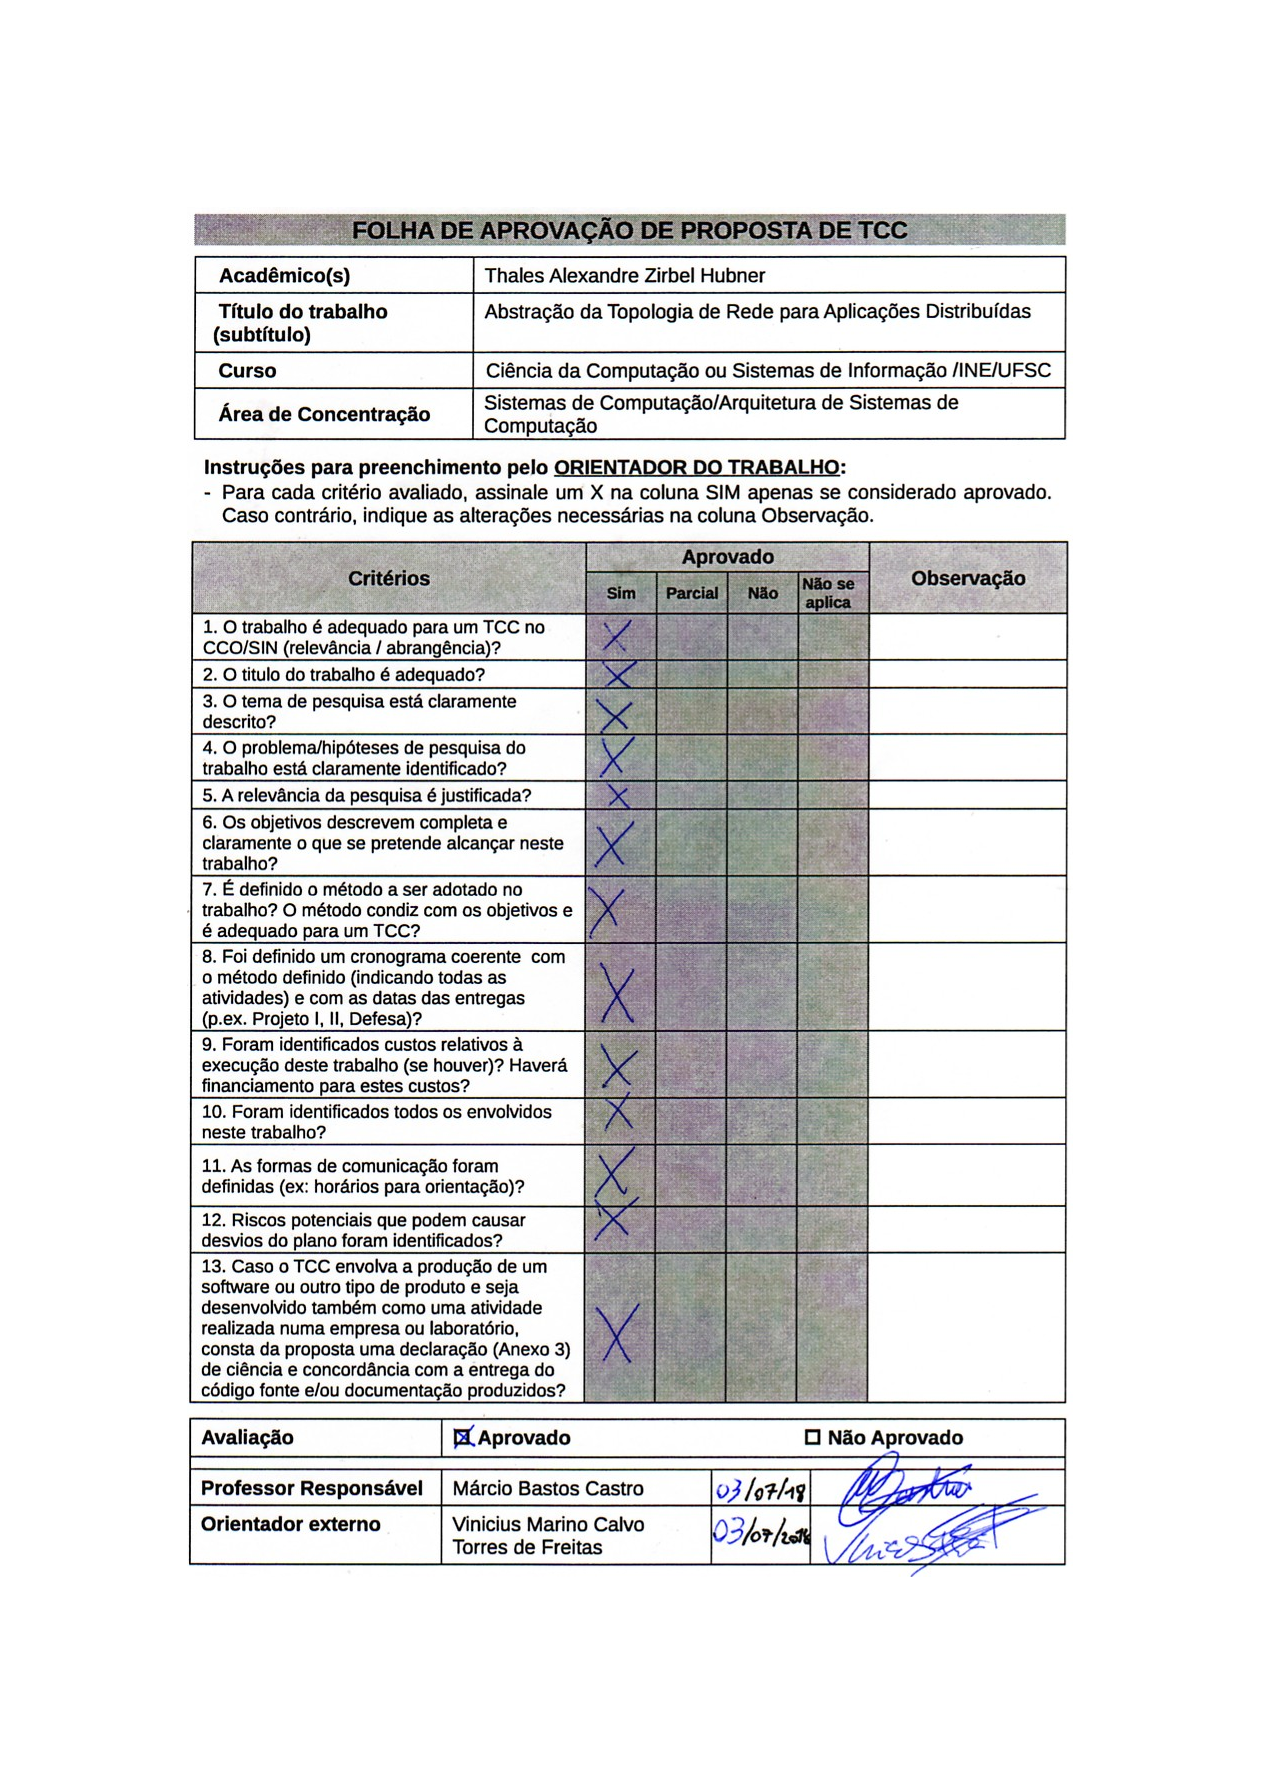
\includepdf{folha_aprovacao_assinada}  
%\end{folhadeaprovacao}
% ---

\begin{agradecimentos}
A minha família, por ter me dado suporte, carinho, felicidade e educação. Sem eles não seria quem sou nem estaria onde estou.

Ao meu orientador e coorientador, por me guiarem, auxiliarem e incentivarem no processo de pesquisa e escrita, por lidarem com meus problemas mais diversos com calma e paciência e por me acompanhar ao longo deste trabalho.

Ao laboratório \textit{Embedded Computing Lab} (ECL) e seus integrantes, pela infraestrutura, pelo apoio, pela compania, pelas ideias e pelas discussões.

A Universidade Federal de Santa Catarina, por oferecer infraestrutura, por ser um ambientes de pesquisa onde pude atuar, por me oferecer um espaço de ensino e crescimento pessoal, sem o qual não teria realizado este trabalho.

A banca, pelas revisões, pelas críticas e pela contribuição a este trabalho.

Ao corpo docente do INE, pelo incentivo, dedicação e auxilio ao seus alunos, por me muniram do conhecimento necessário na área.

Aos meus amigos e colegas de curso, que fizeram minha experiência universitária possível, me auxiliaram em momentos complicados, me mantiveram feliz, me ajudaram a crescer e me trouxeram bem estar e diversão.

E a muitos outros que também suportaram minha qualidade de espirito e de vida mas não foram citados aqui.
\end{agradecimentos}

% ---
% RESUMOS
% ---

% resumo em português
\begin{resumo}

A repartição de trabalho em ambientes distribuídos é um problema relevante em aplicações como simulações sísmicas, dinâmica molecular e previsão de tempo, pois estas possuem comportamento dinâmico, gerando desbalanceamento de carga no sistema. 
Uma das maneiras de resolver esse problema é a utilização de balanceadores de carga dinâmicos, cuja função é reduzir o tempo de execução da aplicação através de uma distribuição de tarefas mais homogênea. 
Uma alocação de tarefas que leva em consideração a topologia da rede pode reduzir latências de comunicação e efeitos de contenção alocando tarefas que se comunicam próximas uma da outra.
Entretanto, poucos balanceadores consideram a topologia do sistema de maneira dinâmica, devido à dificuldade do balanceador de obter informações de topologia de rede, como distância e proximidade de tarefas, e de levá-las em consideração para o remapeamento de tarefas.

Este trabalho desenvolveu a Net Topo, uma abstração da topologia de rede que facilita o acesso a informações de topologia da rede e a utilização destas para distribuição de tarefas.
Ela oferece funções de proximidade e distância entre nós na rede com foco em melhorar a repartição de trabalho.
Foram implementadas algumas opções de inicialização da estrutura e foi proposta uma forma de arquivar a informação de topologia.

A comprovação do funcionamento da Net Topo se deu através de testes com um \textit{benchmark} sintético para balanceamento de carga.
Uma estratégia de balanceamento de carga foi modificada para utilizar a abstração elaborada e, quando comparada com a original, não só teve sobrecusto negligenciável mas apresentou benefícios na inicialização e na velocidade da estrutura.
Por arquivar as informações de topologia para execuções futuras, a Net Topo permitiu uma redução de 97\% no tempo de inicialização de topologia.
O desempenho da abstração foi avaliado em diferentes escalas, mostrando que a Net Topo consegue apresentar boa escalabilidade na maioria das suas funções.

%um parágrafo de fechamento e trabalhos futuros? Não consegui achar um inicio bom para nem conteudo suficiente
% falar sobre charm no resumo?
% a net topo permite expressar uma gam



%  Segundo a \citeonline[3.1-3.2]{NBR6028:2003}, o resumo deve ressaltar o
%  objetivo, o método, os resultados e as conclusões do documento. A ordem e a extensão
%  destes itens dependem do tipo de resumo (informativo ou indicativo) e do
%  tratamento que cada item recebe no documento original. O resumo deve ser
%  precedido da referência do documento, com exceção do resumo inserido no
%  próprio documento. (\ldots) As palavras-chave devem figurar logo abaixo do
%  resumo, antecedidas da expressão Palavras-chave:, separadas entre si por
%  ponto e finalizadas também por ponto.\citeonline{Emma}.\citeonline{Nielsen}.
%  \citeonline{Goodfellow-et-al-2016}

 \vspace{\onelineskip}
    
 \noindent
 \textbf{Palavras-chaves}: topologia de rede. balanceamento de carga. aplicações distribuídas. aplicações paralelas
 
\end{resumo}
\cleardoublepage

% resumo em inglês
% \begin{resumo}[Abstract]
%  \begin{otherlanguage*}{english}
%    This is the english abstract.

%    \vspace{\onelineskip}
 
%    \noindent 
%    \textbf{Key-words}: latex. abntex. text editoration.
%  \end{otherlanguage*}
% \end{resumo}

% ---
% inserir lista de ilustrações
% ---
\pdfbookmark[0]{\listfigurename}{lof}
\listoffigures*
\cleardoublepage
% ---


% ---
% inserir lista de tabelas
% ---
\pdfbookmark[0]{\listtablename}{lot}
\listoftables*
\cleardoublepage
% ---


\addtocontents{loa}{\def\string\figurename{Algorithm}}
\listofalgorithms
\cleardoublepage

% ---
% inserir lista de abreviaturas e siglas
% ---
\begin{siglas}
  \item[PE] \textit{Processing Element}, unidade de processamento
  \item[LB] \textit{Load Balancer}, balanceador de carga
  \item[hwloc] \textit{Portable Hardware Locality}
  \item[netloc] \textit{Portable Network Locality}
  \item[CSC] \textit{Compressed Sparse Columns}
  \item[XML] \textit{Extensible Markup Language}
\end{siglas}
% ---

% ---
% inserir lista de símbolos
% ---
\begin{simbolos}
    \item[$\textbf{S}$] Aceleração
    \item[$n$] Número de núcleos utilizados
    \item[$s$] Parcela paralelizável do programa
    \item[$d$] Número de dimensões da topologia
    \item[$k$] Número de nós por dimensão da topologia
    \item[$p$] Número de nós totais da topologia
    \item[$f$] Valor de \textit{fanout} da árvore
    \item[$h$] Número de \links (conexões) remotos por roteador
    \item[$r$] Número de roteadores por grupo
    \item[$c$] Número de cores por máquina
    \item[$m$] Número de máquinas no sistema
%  \item[$ \Gamma $] Letra grega Gama
%  \item[$ \Lambda $] Lambda
%  \item[$ \zeta $] Letra grega minúscula zeta
%  \item[$ \in $] Pertence
\end{simbolos}
% ---

% ---
% inserir o sumario
% ---
\pdfbookmark[0]{\contentsname}{toc}
\tableofcontents*
\cleardoublepage
% ---



% ----------------------------------------------------------
% ELEMENTOS TEXTUAIS
% ----------------------------------------------------------
\textual


% ----------------------------------------------------------
% Introdução
% ----------------------------------------------------------
\chapter{Introdução}

Este capítulo apresenta o tema de pesquisa do Trabalho de Conclusão de Curso, o escopo no qual o problema em questão será tratado e a justificativa do projeto. 
Na Seção~\ref{sec:introducao} é apresentado o contexto e a motivação para a realização do trabalho. 
Na Seção~\ref{sec:objetivos} são introduzidos os objetivos gerais e específicos, as restrições e premissas existentes, a lista de marcos e os critérios de aceite do projeto. 
Na Seção~\ref{sec:metodologia}, são abordados os métodos de pesquisa envolvidos para alcançar a solução proposta.
Uma visão geral do restante do trabalho é indicada na Seção~\ref{sec:organização}.


\section{Motivação}
\label{sec:introducao}

Aplicações no âmbito científico e industrial incluem cada vez mais detalhes, demandam precisão ainda maior e/ou possuem uma complexidade muito elevada, criando uma demanda cada vez maior por poder de processamento~\cite{pilla-thesis}. Uma das maneiras utilizadas para suprir esta demanda é com computação paralela, que soluciona estes problemas através da repartição de trabalho entre unidades de processamento (\textit{Processing Elements} ou PEs) e a execução destas parcelas simultaneamente. Este método permite que um aumento no número de PEs leve a uma redução no tempo da aplicação. Contudo a melhoria no tempo é limitada pela parcela não paralelizável do programa e pelos recursos do sistema~\cite{amdahl}. 

% Supercomputadores que utilizam da computação paralela foram criados para alcançar processamento massivo e por décadas estas máquinas cresceram. Elas alcançaram um ponto onde se percebeu que velocidade e poder de processamento não eram as métricas adequadas para desempenho destas máquinas. Estes computadores consomem uma quantidade tremenda de energia que é em maior parte dissipada, se transformando em grandes geradores de calor~\cite{green500}. A geração de calor excessiva é um problema em sistema pois temperaturas altas aumentam sua chance de falha e tempo fora de operação~\cite{efficient-metric}. Como contramedida é necessário a implantação de um sistema eficiente de redução de temperatura, que traz outro grande sobrecusto de energia. Com estes problemas em mente a métrica pensada para estas máquinas é a eficiência de processamento, que leva em conta a energia gasta no sistema, a velocidade e o poder de processamento~\cite{efficient-metric}.

Uma das opções para obter eficiência de processamento é o uso de um número maior de núcleos menos potentes~\cite{snir-encyclopedia}. A organização de um número grande de PEs acaba levando a um sistema com memória distribuída, que operam com o uso de diversas máquinas e utilizam alguma rede para a interligação e comunicação. A escolha destes sistemas é devida ao seu custo baixo e a sua grande escalabilidade através do aumento no número de máquinas. O contraponto destas vantagens é o desenvolvimento destas aplicações, que se torna mais complexo pois tem de levar em consideração fatores impactantes como sincronização, dependência e distribuição de dados, balanceamento de carga e custos de comunicação~\cite{pilla-thesis}.

A comunicação em um sistema é realizado através de \links (ligações) entre PEs. Estas ligações estão dispostas utilizando algum padrão de topologia, como malhas, tori, \fatts ou \dgfly, que buscam otimizar alguma característica da rede, como custo de implantação, tráfego ou latência média. 
A alocação de tarefas nestes sistemas geralmente ocasiona um uso compartilhado de \links por múltiplos núcleos, que pode saturar partes da rede devido a uma carga maior de informação a ser transmitida do que os \links suportam, resultando em contenção~\cite{bhatele-encyclopedia}. 
Outro fator de topologia que impacta o desempenho da aplicação é a possibilidade da rede ter ligações com custos heterogêneos~\cite{dragonfly}, tendo latências diferentes para \links diferentes.

%old:  Os PEs em sistemas distribuídos se comunicam usando diversas topologias de rede, como malhas, tori, \fatts ou \dgfly. Os núcleos utilizam de \textit{links} de conexão da rede para efetuar comunicação no sistema. O compartilhamento destes pode resultar em congestão, um congestionamento da rede devido ao sobreuso de alguns \links~\cite{bhatele-encyclopedia}. Outro fator é a possibilidade da rede não ter ligações com custos iguais de comunicação~\cite{dragonfly}, tendo variações de latência e velocidade em partes distintas da rede. O impacto disto é que os caminhos menos custosos entre PEs na rede nem sempre são os menores em questão de \links percorridos.

A repartição de trabalho em ambientes paralelos é um problema a ser tratado, pois aplicações como simulações sísmicas~\cite{dupros,tesser}, dinâmica molecular~\cite{bhatele-kale} ou previsão de tempo~\cite{rodrigues} possuem comportamento dinâmico, ou seja suas cargas mudam ao longo da execução da aplicação, levando um mapeamento homogêneo de tarefas a um estado desbalanceado do sistema, resultando em uma diferença de carga entre alguns PEs. 
Esta diferença faz com que alguns PEs não tenham trabalho para executar enquanto esperam a conclusão de tarefas nos PEs mais carregados, reduzindo o desempenho geral da aplicação. 
Para consertar tais desvios pode-se usar um balanceador de carga (\textit{Load Balancer} ou LB) dinâmico, cujo trabalho é remapear as tarefas entre os PEs, buscando um estado mais balanceado do sistema. 
Este rearranjo garante a utilização dos PEs de maneira mais homogênea e leva a uma redução do tempo da aplicação pela redução de tempo ocioso.

Os caminhos utilizados dentro de uma rede impactam o tempo de execução de um programa, pois caminhos mais lentos resultam em uma latência maior de comunicação e problemas como contenção. É possível que aplicações e LBs levem em conta os custos de comunicação entre os PEs e os custos de movimentação destas tarefas dentro da rede. Tal abordagem pode levar a uma redução do custo de comunicação, evitando a troca de informação e tarefas através de partes lentas da rede. Uma abstração da topologia de rede que permita fácil acesso às informações da rede e de comunicação reduziria a complexidade de criação de aplicações que lidam com contenção e latência.
% olhar netloc para referencia

\textit{Hardware Locality} (\hwloc) e \textit{Network Locality} (\netloc) são duas ferramentas que fornecem uma abstração da topologia para aplicações.
Ambas coletam diversas informações de um sistema, realizam uma interpretação intermediária e a disponibilizam para um usuário, de maneira visual ou em um arquivo \textit{Extensible Markup Language} (XML).
O \hwloc apanha somente a parte de topologia de máquina, enquanto o \netloc coleta informações da rede.
Nenhuma das duas visa auxiliar alocação de tarefas com funções para cálculo de proximidade ou distâncias.
Este trabalho desenvolveu a Net Topo, uma abstração de topologia com foco em auxiliar na alocação de tarefas, detalhado adiante.

\section{Objetivos}
\label{sec:objetivos}

Os objetivos deste trabalho são de desenvolver e avaliar uma abstração da topologia de rede, permitindo seu uso para balanceadores de carga e aplicações distribuídas. Para este fim, seguem os objetivos específicos:

\begin{enumerate}
\item Desenvolver uma API de acesso à informações de topologia de rede;
\item Implementar algoritmos e estruturas para o uso destas informações;
\item Desenvolver uma interface desta abstração utilizando a plataforma Charm++~\cite{website:CHARM};
\item Modificar um LB para que utilize esta base, visando a prova funcional da abstração.

\end{enumerate}

% \begin{flushleft}
% \textbf{Premissas:}
% \begin{itemize}
% \item Um computador estará disponível para realização do trabalho; 
% \item O orientador terá disponibilidade para reuniões periódicas;
% \item Disponibilidade de energia e internet.
% \item Acesso a uma máquina com uma topologia diferenciada para a realização dos testes.
% \end{itemize}

% \textbf{Marcos:}
% \begin{itemize}
 
% \item Entrega do resumo em TCC I: 4ª semana de Novembro/2018; 
% \item Entrega da abstração implementada: 4ª semana de Janeiro/2018;
% \item Entrega da interface com \charm: 1ª semana de Abril/2019;
% \item Entrega do Balanceador modificado: 4ª semana de Abril/2019;
% \item Entrega da primeira versão da monografia em TCC II: inicio da 3ª semana de Junho/2019; 
% \item Defesa da monografia: 1ª semana de Julho/2019;
% \item Entrega da versão final da monografia em TCC II: 4ª semana de Julho/2019.
% \end{itemize}

% \textbf{Critérios de aceite:}
% \begin{itemize}
% \item Aprovação da banca avaliadora;
% \item Aprovação do orientador;
% \item Aprovação do coorientador;
% \item Conformidade da monografia com as normas definidas pela instituição;
% \item Prazos cumpridos.
% \end{itemize}
% \end{flushleft}

\section{Método de Pesquisa}
\label{sec:metodologia}

 
Inicialmente, este trabalho de conclusão foi dividido em duas partes principais: uma de cunho teórico, onde foram estudados os conceitos básicos e o estado da arte para o projeto, e outra mais prática, que envolveu o aprendizado do \textit{framework} \charm. 
A primeira parcela foi constituída por um estudo sobre topologia de rede e balanceamento de carga em aplicações paralelas, criando uma base de conhecimentos para o projeto. 
A segunda parte teve foco no entendimento da plataforma e suas nuances, visando facilitar a implementação da abstração.

A criação da abstração da topologia de rede utiliza a linguagem de programação C++ e é posteriormente inicializada manualmente ou com informações do \fw de programação paralela \charm~\cite{website:CHARM}. 
Esta plataforma possui uma base sólida para a criação, utilização e teste de balanceadores de carga e outras aplicações paralelas~\cite{bhatele-thesis}. 
Além disto, \charm contém somente abstrações de topologia fixas (detalhado na seção~\ref{sec:charm}), carecendo de uma abstração elaborada da topologia de rede, proposta neste trabalho.

Para a criação da abstração de topologia de rede, foi criada uma especificação de suas funções e suas estruturas, criando um esqueleto que foi preenchido posteriormente. 
Um estudo de estruturas e algoritmos utilizados no estado da arte foi realizado para observar como tais funções podem ser implementadas de maneira eficiente.

Após a implementação dos algoritmos e estruturas da abstração de topologia de rede, foi implementado um método de inicialização da estrutura através do \fw \xspace \charm, que coleta as informações necessárias para a execução de seu \textit{runtime}.
Além da inicialização utilizando o \charm, foi implementado uma inicialização utilizando XML e uma inicialização manual.
Para cobrir o funcionamento das funções da abstração independente da forma de inicialização, foram realizados testes de unidade utilizando \textit{Gtest}.

O balanceador de carga \textit{NeighborLB} foi modificado para utilizar esta abstração de rede, demonstrando seu funcionamento e sua utilidade através das funções implementadas e utilizadas.
O balanceador foi comparado com o original, verificando o sobrecusto da abstração criada.

Na última etapa deste trabalho foram realizados testes de desempenho dos algoritmos de inicialização, serialização, proximidade, \hops e distância, avaliando o seu desempenho relativo a entradas diferentes.

\section{Organização do Trabalho}
\label{sec:organização}

O restante do trabalho é dividido em quatro capítulos.
O Capítulo~\ref{cap:conceituacao} apresenta alguns conceitos de importância para o trabalho e duas abstrações de topologia existentes.
No Capítulo~\ref{cap:proposta} a abstração Net Topo é apresentada, incluindo detalhes da estrutura, das funcionalidades e da implementação.
O Capítulo~\ref{cap:comprovacao} descreve um balanceador de carga modificado e os testes realizados para comprovar o funcionamento da abstração e avaliar sua escalabilidade.
O último capítulo apresenta uma conclusão e possíveis trabalhos futuros.
O código implementdo pelo trabalho pode ser encontrado em \href{https://github.com/Thaleszh/Net-Topo}{https://github.com/Thaleszh/Net-Topo}.
% No final do trabalho estão os apêndices com os códigos realizados para este de trabalho.
% O Apêndice~\ref{apd:net_topo} contêm os códigos da abstração e das estruturas que ela utiliza.
% No Apêndice~\ref{apd:testes} estão os testes de unidade e no Apêndice~\ref{apd:lb} os codigos do balanceador modificado, myNeighborLB.


% ----------------------------------------------------------
% PARTE - preparação da pesquisa
% ----------------------------------------------------------
% \part{Preparação da pesquisa}

% ----------------------------------------------------------
% Capitulo com exemplos de comandos inseridos de arquivo externo 
% ----------------------------------------------------------

\include{abntex2-modelo-include-comandos}

% ----------------------------------------------------------
% Parte de revisão de literatura
% ----------------------------------------------------------
% \part{Revisão de Literatura}

% ---
% Capitulo de revisão de literatura
% ---

\chapter{Fundamentação Teórica}
\label{cap:conceituacao}

O desempenho de um aplicação paralela depende de uma multitude de fatores como \textit{hardware}, técnicas de otimização, topologia, arquitetura utilizada, políticas tomadas e comunicação. Na Seção~\ref{sec:parellel} são abordadas questões relacionadas a computação paralela, incluindo algumas de suas características e alguns de seus limites. A Seção~\ref{sec:topologia} aborda topologias de sistemas paralelos, suas características, seu impacto na aplicação e algumas abstrações de topologia disponíveis. Na Seção~\ref{sec:lb} é tratado o que é um balanceador de carga, que problemas estes buscam resolver e os benefícios de um balanceador ciente de topologia.


\section{Computação Paralela}
\label{sec:parellel}

Uma aplicação paralela realiza computação de maneira concorrente, utilizando os recursos de processamento disponíveis simultaneamente para a realização destas tarefas. O ganho de desempenho ao se realizar tarefas simultaneamente é pago com uma complexidade maior de \textit{hardware}, arquiteturas e com a necessidade de sincronização, garantias de exclusão, trocas de mensagem e outras técnicas de programação e compilação~\cite{david-encyclopedia}.

O fim da lei de Moore~\cite{patterson} e o limite da barreira de potência tornou a redução dos transistores e o aumento na frequência dos processadores insuficiente, abrindo um espaço para os ganhos de arquiteturas paralelas~\cite{tanenbaum:operational_systems}. Em ambientes de múltiplos núcleos se utiliza um número maior de núcleos menos poderosos, em busca de eficiência através de um paralelismo maior e de um consumo de energia mais baixo~\cite{snir-encyclopedia}. Estes sistemas são facilmente escalados através da inclusão de mais núcleos e extensão da rede, mas agregam uma série de complexidades para o desenvolvimento devido a outros fatores, como sincronização, dependência e distribuição de dados, balanceamento de carga e custos de comunicação entre os núcleos~\cite{pilla-thesis}.

A relação entre a aceleração de uma aplicação $(\textbf{S})$ com o número de núcleos utilizados ($n$) e sua parcela paralelizável ($s$) é expressa pelo argumento de Amdahl na Equação~\ref{eq:amdahl}~\cite{amdahl}. É importante constatar que são desconsiderados detalhes como os custos de acesso a memória, envio de mensagens, geração de \textit{threads} e latência de interconexão. A fórmula é então utilizada como uma estimativa otimista para a aceleração e não como uma referência exata, pois o impacto exato não é simples de calcular e pode ser afetado por diversos fatores externos a execução.

\begin{equation}
\textit{\textbf{S}} = \frac{1}{(1-\textit{s}) + \frac{\textit{s}}{\textit{n}}}
\label{eq:amdahl}
\end{equation}

Na Equação~\ref{eq:amdahl}, quando $n$ tende ao infinito a equação indica um limite na aceleração de acordo com a parcela serial do programa $(1-s)$, pois esta não se beneficia da paralelização. 
Levando este limite em conta, as aplicações paralelas muitas vezes são adaptadas para que sua parte paralelizável inclua mais detalhes ou mais precisão, fazendo com que um aumento no número de PEs leve a mais informação sendo processada e não a uma aceleração~\cite{gustafson}.

\subsection{Carga e Comunicação}

O processamento a ser realizado em uma aplicação paralela é dividido em tarefas e em cargas. 
A carga representa a quantidade de processamento que uma tarefa precisa realizar em um único PE. 
Em um sistema paralelo, múltiplas tarefas são executadas simultaneamente, tendo sua carga distribuída entre os PEs do sistema. 
Um núcleo que possui uma carga maior que um limiar acima da média é considerado sobrecarregado, e um núcleo que tem menos carga que um limiar abaixo da media é considerado subcarregado. 
Esta diferença nas cargas faz com que alguns PEs não tenham trabalho para executar enquanto esperam a conclusão de tarefas nos PEs mais carregados, sub-utilizando o sistema. 
Esta situação é chamada de desbalanceamento.

\begin{figure} [b]
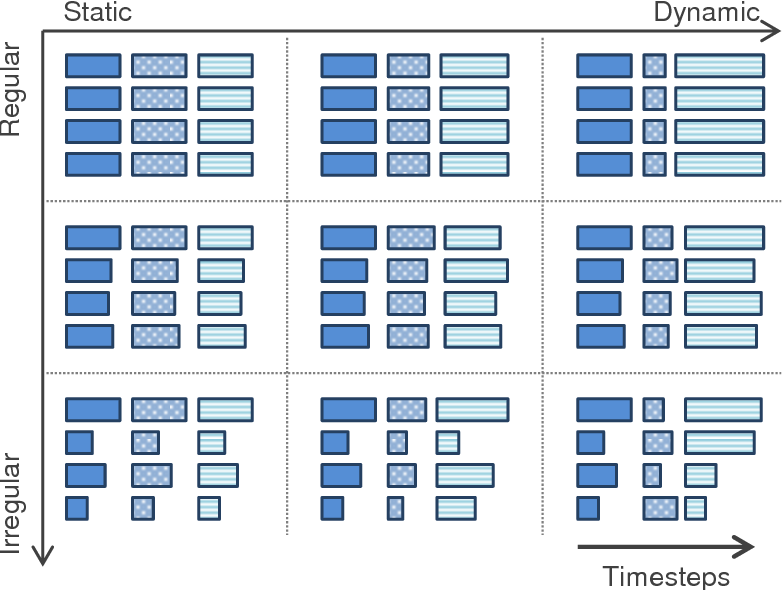
\includegraphics[width=0.62\textwidth]{load_pilla}
\centering
\caption[Diferentes graus de regularidade e dinamicidade em relação a carga de uma aplicação.]{Diferentes graus de regularidade e dinamicidade em relação a carga de uma aplicação ~\cite{pilla-thesis}.}
\label{fig:load}
\end{figure}

Em aplicações paralelas, a carga de cada tarefa e sua comunicação pode ser diferente das demais tarefas. Essas diferenças podem se manter constantes ou até mesmo variar ao longo da execução da aplicação paralela. 
Duas características refletem isso: a \textit{regularidade} e a \textit{dinamicidade}. 
A regularidade de uma aplicação reflete o quanto a carga ou a comunicação de uma tarefa difere de uma outra tarefa. Uma aplicação com carga ou comunicação regular tem cargas ou comunicação aproximadamente iguais. 
Quando a carga ou comunicação difere entre tarefas, a aplicação tem carga ou comunicação irregular, respectivamente.
A dinamicidade de uma aplicação indica o quanto a comunicação ou carga de uma tarefa muda ao longo do tempo. Quando sua carga ou comunicação não muda ao longo do tempo, é dita estática e quando muda, é dita dinâmica~\cite{pilla-thesis}.
As Figuras~\ref{fig:load} e \ref{fig:communication} apresentam a variação de regularidade e dinamicidade em relação a carga e a comunicação de uma tarefa, respectivamente. 

\begin{figure} [h]
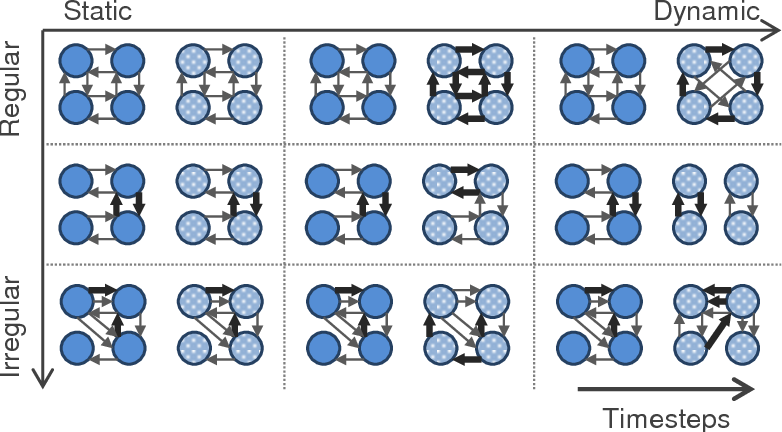
\includegraphics[width=0.67\textwidth]{comm_pilla}
\centering
\caption[Diferentes graus de regularidade e dinamicidade em relação a comunicação de uma aplicação.]{Diferentes graus de regularidade e dinamicidade em relação a comunicação de uma aplicação ~\cite{pilla-thesis}.}
\label{fig:communication}
\end{figure}

A distribuição de tarefas em um ambiente paralelo deve levar em consideração sua regularidade e dinamicidade. 
Técnicas de escalonamento, alocação de tarefas e balanceamento de carga são utilizadas para gerenciar e dispor as tarefas de maneira eficiente no sistema. 
Na Seção~\ref{sec:lb} serão abordadas algumas técnicas de balanceamento de carga.

\subsection{Computação Distribuída}

Em ambientes multiprocessados, existe algum dispositivo de memória compartilhada entre todos os PEs, o qual é organizado de forma a impedir problemas de coerência e consistência. \textit{Chips} \textit{multicore} e \textit{manycore} são exemplos de ambientes multiprocessados. 
Ambientes multiprocessados não escalam bem devido à complexidade de arquitetura e custos de produção, abrindo espaço para ambientes multicomputados. 
Em ambientes multicomputados a memória não é compartilhada entre todos os PEs e algum meio de interconexão é utilizado para realizar as trocas de informação, mas o sistema ainda é organizado de maneira similar~\cite{tanenbaum:operational_systems}.

Em um sistema distribuído, computadores com diferentes arquiteturas, organizações, locais e comportamentos podem ser interconectados em uma mesma rede e utilizados em conjunto. 
Devido à alta independência dos componentes, estes sistemas são altamente escaláveis através da adição de computadores e expansão da rede. 
A comunicação e coordenação destes sistemas se torna muito mais complexa e custosa devido ao número de componentes, precisando ser tratada com mais detalhe~\cite{tanenbaum:operational_systems}.


\section{Topologia de Rede}
\label{sec:topologia}

Sistemas paralelos utilizam redes de interconexão para efetuar a comunicação entre seus PEs. 
Estas redes têm propriedades como diâmetro, distância média, grau, latências e largura de banda que regem a comunicação dentro da rede. 
O padrão de interconexões entre PEs é chamado de topologia e esta pode assumir diversas formas como malhas, tori e \textit{fat-trees}.

As topologias de uma rede podem ser dividas em duas categorias: \textit{diretas} e \textit{indiretas}. 
Em redes diretas, os PEs são conectados diretamente  uns aos outros através de \links. Para que uma mensagem possa ser transmitida de um PE a outro, esta precisa trafegar através de vários destes \links.
O cruzamento de um \link é chamado de \hop e a distância entre um ponto a outro na rede pode ser definido pelo número de \hops realizados. 
Malhas, tori e hipercubos são exemplos de redes diretas. 
Em redes indiretas, PEs são conectados a \switches (roteadores) que roteiam as mensagens. Nenhum PE é ligado diretamente a outro PE e portanto é necessário cruzar dois ou mais \switches para alcançar outro PE. 
\Fatts e \dgfly são exemplos de redes indiretas~\cite{bhatele-encyclopedia}.

A hierarquia é um fator presente em algumas topologias indiretas, como \fatt e \dgfly, e divide esta em níveis de proximidade. 
Cada nível de hierarquia na topologia representa um agrupamento diferente da rede. 
Redes hierárquicas apresentam pontos de gargalo de tráfego entre seus níveis e requerem uma replicação de \links para que isto não se torne um problema.

Uma rede de interconexão tem duas propriedades importantes que afetam sua comunicação: \textit{simetria} e \textit{uniformidade}. 
Um nível de topologia é dito simétrico quando o tempo de comunicação de um ponto A para um ponto B é o mesmo que de B para A. Caso contrário, este é dito assimétrico. 
Um nível de topologia é uniforme quando todos os PEs neste nível tem o mesmo tempo de comunicação entre si~\cite{pilla-thesis}. 
Nesse sentido, uma rede indireta pode se tornar assimétrica devido ao roteamento de informações. 
%problema: parece estar mal formulado e estranho porque por exemplo de p1 a p3 pode ter um caminho mais longo (tori por exemplo)
%problema tem alguma utilidade falar isso?

\begin{figure} [b]
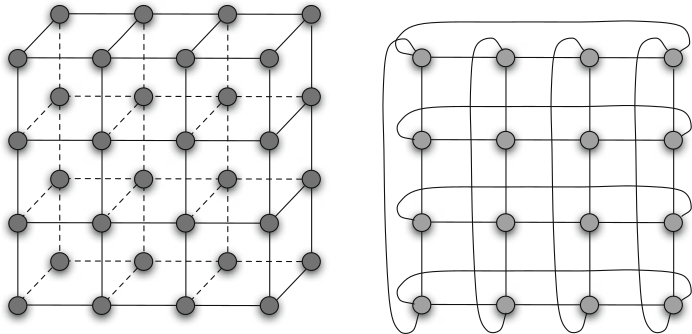
\includegraphics[width=0.5\textwidth]{mesh_torus}
\centering
\caption[Uma malha de dimensões (4,4,2) e uma torus 2D]{Uma malha de dimensões (4,4,2) a esquerda e uma torus 2D a direita~\cite{bhatele-encyclopedia}}
\label{fig:mesh_torus}
\end{figure}

Algumas métricas são utilizadas para observar o comportamento de uma rede, como o diâmetro, o número de \links, o grau e a bisseção de \links. 
O diâmetro de uma rede é definido como sendo o maior caminho dentre os caminhos mais curtos que ligam quaisquer dois nós da topologia. Usualmente, as distâncias são medidas através do número de \hops, sendo esta métrica também utilizada para determinar a maior latência dentro de uma rede. 
O número de \links apresenta a quantidade total de \links dentro da rede, uma informação usada para avaliar o custo de implantação. 
O grau de uma rede é o número de \links conectados em cada nó da rede. 
A bisseção da largura de banda representa a quantidade de \links entre duas partes da rede, partida de modo a gerar o mínimo de \links entre duas metades da rede. 
Essa métrica é utilizada para estimar o quanto de tráfego a rede suporta~\cite{david:paralel}. A seguir, são apresentadas algumas topologias abordadas neste trabalho.

\begin{figure} [t]
    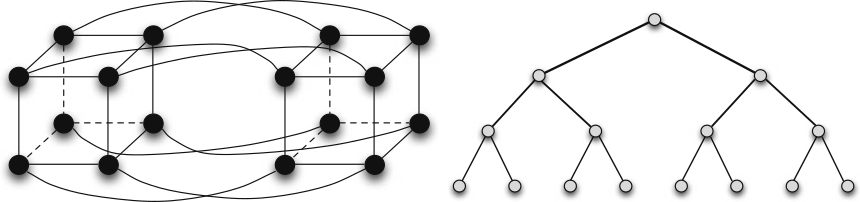
\includegraphics[width=0.7\textwidth]{hypercube_fat_tree}
    \centering
    \caption[Um hipercubo de e uma \fatt]{Uma rede direta em forma de hipercubo de 4 dimensões a direita e uma indireta em forma de \fatt binária com 4 níveis a esquerda~\cite{bhatele-encyclopedia}}
    \label{fig:cube_fat}
\end{figure}

\begin{figure} [t]
    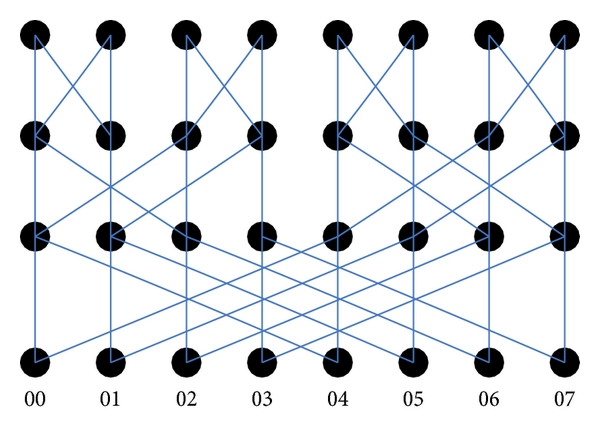
\includegraphics[width=0.4\textwidth]{bfly}
    \centering
    \caption[Uma rede \textit{Buttefly}]{Uma rede \textit{butterfly} de 3 níveis e 8 nós~\cite{Liu:bfly}}
    \label{fig:bfly}
\end{figure}

\begin{itemize}
    \item \textbf{Malha}: Uma topologia direta similar a uma matriz de múltiplas dimensões, onde cada \link só cruza uma dimensão da rede e na menor distância possível ~\cite{Solihin}.
    Malhas podem ser dispostas em diversas dimensões. A Figura~\ref{fig:mesh_torus} representa uma malha de dimensões 4, 4 e 2.
    
    \item \textbf{Torus}: Uma malha com um \link entre nodos finais de cada dimensão da rede, reduzindo o diâmetro da rede e aumentando sua bisseção. 
    Uma torus de dimensões 4 e 4 pode ser observada na Figura~\ref{fig:mesh_torus}.
    
    \item \textbf{Hipercubo}: Uma malha com 2 nodos em cada dimensão.
    Um hipercubo visa reduzir a distancia máxima da rede. 
    A Figura~\ref{fig:cube_fat} mostra um exemplo de hipercubo.
    
    \item \textbf{\Fatt}: Uma topologia de rede indireta em forma de árvore, onde \links em níveis mais altos possuem mais largura de banda. 
    Esta topologia é encontrada como topologia interna de máquinas. 
    Uma \fatt é representada na Figura~\ref{fig:cube_fat}.
    
    \item \textbf{\textit{Butterfly}}: Uma topologia indireta que visa escalabilidade e redução de distâncias através da replicabilidade de \links e de roteadores.
    É utilizada para gerar uma bisseção de banda elevada dentro de uma rede.
    Sua desvantagem é o grande número de \links, o qual é muito superior ao de outras topologias~\cite{david:paralel}.
    
    \item \textbf{\Dgfly}: Uma topologia indireta que cria agrupamentos de roteadores em grupos distintos, visando reduzir o número de \links da rede para reduzir seu custo.
   
    
    \item \textbf{\textit{Slim Fly}}: Uma topologia indireta similar a \dgfly mas otimizada matematicamente, reduzindo o custo e energia gasta enquanto aumenta a resiliência da rede em relação à falha de \links~\cite{slimfly}.
\end{itemize}

\setlength{\tabcolsep}{0.5em}
\begin{table}[t]
    \centering
    \begin{tabular}{c l}
        \toprule
        \textbf{Símbolo} &    \textbf{Descrição}  \\ \midrule
        $d$ & Número de dimensões da topologia.  \\ %\hline
        $k$ & Número de nós por dimensão da topologia.  \\ %\hline
        $p$ & Número de nós totais da topologia.  \\ %\hline
        $f$ & Valor de \textit{fanout} da árvore.  \\ %\hline
        $h$ & Número de \links remotos por roteador \\ %\hline
        $r$ & Número de roteadores por grupo \\ \bottomrule
    \end{tabular}
    \caption[Símbolos utilizados na Tabela~\ref{tab:topo_comparison}]{Símbolos utilizados na Tabela~\ref{tab:topo_comparison}.}
    \label{tab:topo_symbols}
\end{table}

\setlength{\tabcolsep}{0.5em}
\renewcommand{\arraystretch}{1.1}
\begin{table}[t]
    \centering
    \begin{tabular}{l c c c c}
        \toprule
        \textbf{Topologia} &    \textbf{Diâmetro} &  \textbf{Bisseção} &   \textbf{\Links} &     \textbf{Grau} \\ \midrule
        Malha 2-D & $2\sqrt{p}-1$ & $\sqrt{p}$ &   $2\sqrt{p} \times (\sqrt{p}-1)$ &    $2d$  \\ %\hline
        Malha K-D & $dk-1$ & $k^{d-1}$ &   $dk^{d-1} \times (k-1)$ &    $2d$  \\ %\hline
        Tori  & $\frac{dk}{2}-1$ & $k^d$ & $dk^d$ &  $2d$  \\ %\hline
        Hipercubo &  $\log_2 p$ & $\frac{p}{2}$ &  $log_2 p \times \frac{p}{2}$  &  $\log_2 p$  \\ %\hline
        \Fatt &  $2 \times \log_f p$ & $\frac{p}{2}$ & $f(p-1)$ &  $f + 1$  \\ %\hline
        \textit{Butterfly} & $\log_2 p$ & $\frac{p}{2}$ &  $2p \times \log_2 p$ &  $4$  \\ %\hline
        \Dgfly & $3$  & $h((r+2)^2/4) $  &  $ r\times(r-1) +rh  $ & $r + h$ \\ 
        \textit{Slim Fly} & $2$  & - &  $2\times r\times(r-1)$ & $r + h$ \\\bottomrule
    \end{tabular}
    \caption[Diâmetro, bisseção de \links, número \links e grau das topologias de Malha, Tori, Hipercubo, \Fatt, \textit{Butterfly}, \Dgfly e \textit{Slim Fly}.]{Diâmetro, bisseção de \links, número de \links e grau das topologias Malha, Tori, Hipercubo, \Fatt, \textit{Butterfly}, \Dgfly~\cite{li:dgfly} e \textit{Slim Fly}. Os símbolos utilizados são apresentados na Tabela~\ref{tab:topo_symbols}. Adaptado de ~\cite{Solihin}. A topologia \textit{Slim Fly} não apresenta uma fórmula de bisseção, pois ela é calculada aproximadamente utilizando um particionador. Sua bisseção é maior que uma \dgfly mas menor que de um hipercubo~\cite{slimfly}.}
    \label{tab:topo_comparison}
\end{table}

A Tabela~\ref{tab:topo_comparison} apresenta algumas topologias e suas características principais: diâmetro, bisseção, \links e grau. Os símbolos utilizados são descritos na Tabela~\ref{tab:topo_symbols}.
É importante ressaltar que $p = dk$ nas topologias de Malha ou Tori.
Na Tabela~\ref{tab:topo_example} são comparadas topologias com $2^{16}$ nós.
A topologia \dgfly se destaca, pois tem \links com latências diferentes e custos de implementação diferentes, fazendo com que métricas baseadas em \hops e número de \links não reflitam a distância e o desempenho da rede.


\setlength{\tabcolsep}{0.5em}
\begin{table}[t]
    \centering
    \begin{tabular}{l c c c c}
        \toprule
        \textbf{Topologia} &    \textbf{Diâmetro} &  \textbf{Bisseção} &   \textbf{\Links} &     \textbf{Grau} \\ \midrule
        Malha 4D & $63$ & $4096$ & $245760$ &  $8$  \\ %\hline
        Tori 4D & $31$ & $65536$ & $262143$ &  $8$  \\ %\hline
        Hipercubo &  $16$ & $32768$ &  $524288$  &  $16$  \\ %\hline
        \Fatt &  $16$ & $32768$ & $262143$ &  5  \\ %\hline
        \textit{Butterfly} & $16$ & $32768$ &  $2097152$ &  $4$  \\ %\hline
        \Dgfly & $3$  & $4225$  &  $ 16896 $ & $129$ \\
        \textit{Slim Fly} & $3$  & $4225$  &  $ 16896 $ & $129$ \\ \bottomrule
    \end{tabular}
    \caption[Diâmetro, bisseção de banda, número de \links e grau das topologias com 64000 nodos.]{Diâmetro, bisseção de banda, número de \links e grau das topologias de Malha 4D, Tori 4D, Hipercubo, \Fatt de \textit{fanout} 4, \textit{Butterfly} e \Dgfly, todas com $2^{16}$ (65536) nodos.}
    \label{tab:topo_example}
\end{table}


Conforme cresce o número de PEs de um sistema, o fluxo de informação na rede aumenta e mais recursos de rede (\links e \switches) são compartilhados e disputados pelos PEs.
Este compartilhamento pode levar a um problema chamado de contenção, onde a latência da rede aumenta devido a saturação dos \links.
Um mapeamento de tarefas ciente de topologia de rede pode reduzir o compartilhamento de recursos de rede e portanto melhorar o desempenho da aplicação~\cite{bhatele-encyclopedia}.

\begin{figure} [h]
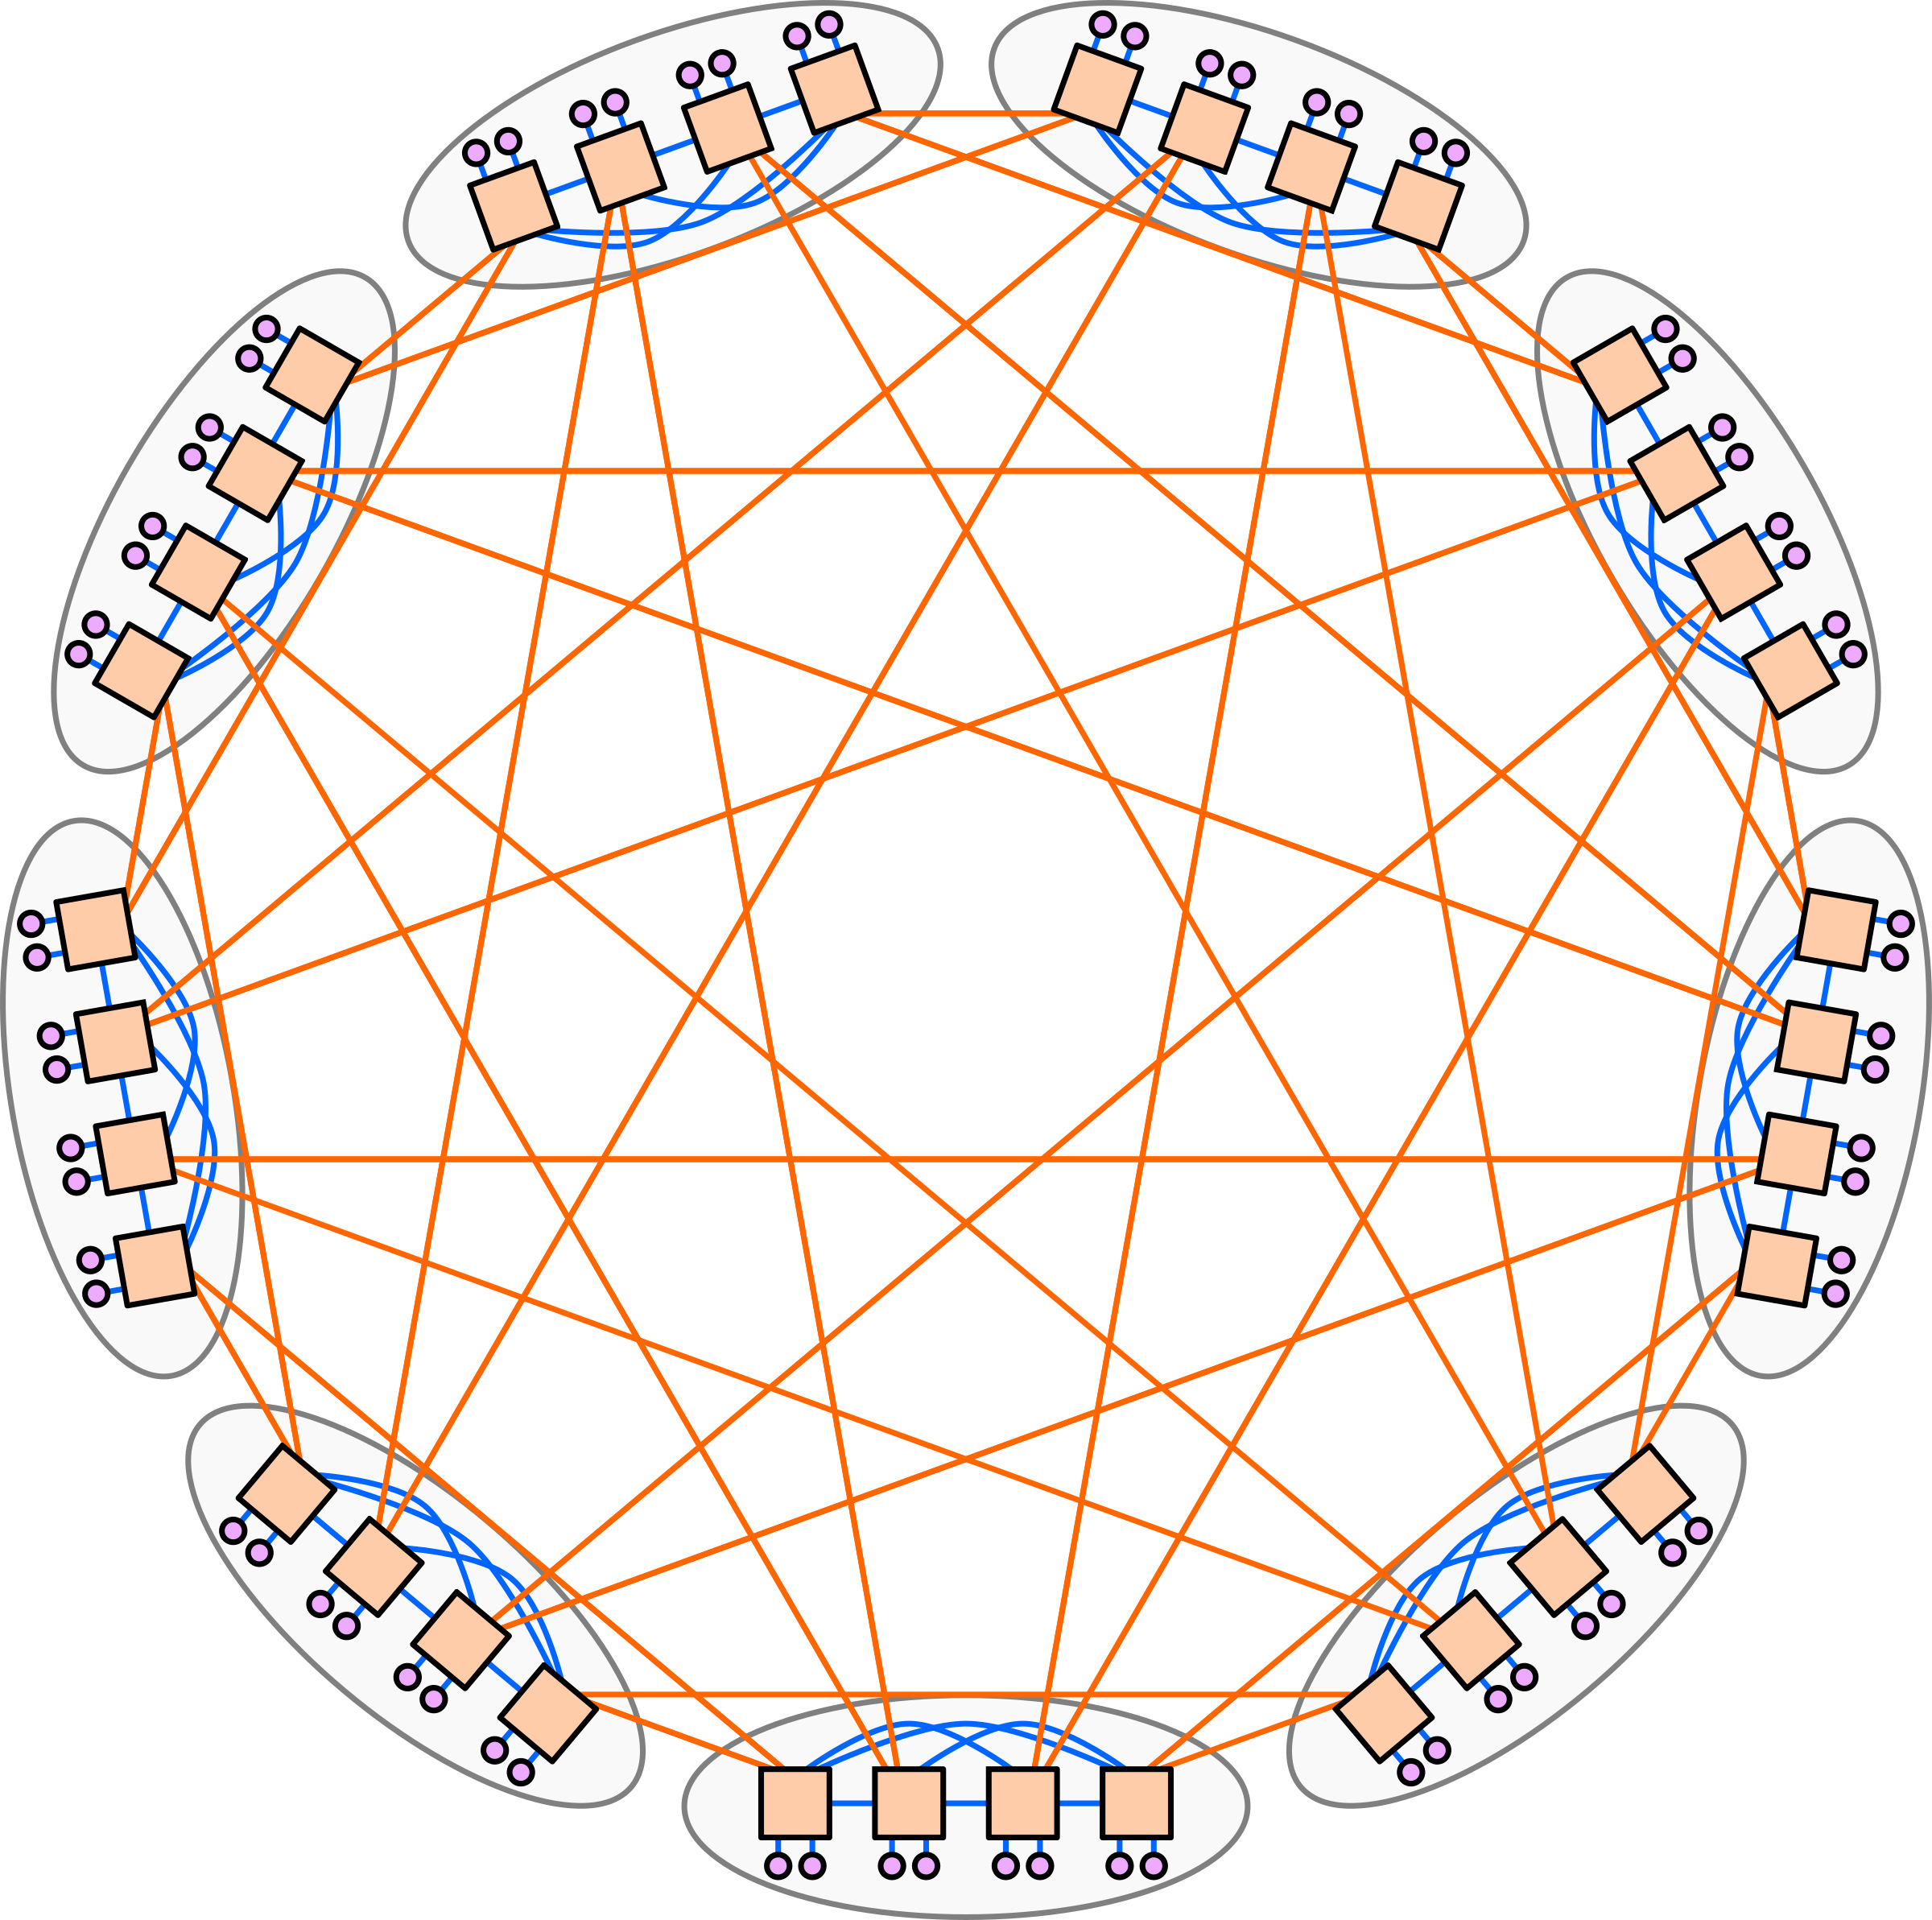
\includegraphics[width=0.6\textwidth]{dragonfly}
\centering
\caption[Um exemplo de rede \dgfly.]{Um exemplo de rede \dgfly. Roteadores e \links globais em laranja, nós em vermelho e \links locais em azul. Fonte: Openclipart, \url{https://openclipart.org/detail/291507/dragonfly-network-topology}, acessado em 08 nov. 2018}
\label{fig:dgfly}
\end{figure}

Topologias de rede podem ter agrupamentos de máquinas interligados com \links de maior latência ou menor capacidade, como, por exemplo, a \dgfly da Figura \ref{fig:dgfly}.
A contenção e a alocação de tarefas neste tipo de rede afeta severamente seu desempenho.
Nestas redes, uma política adequada de roteamento, de alocação de tarefas, de migração de tarefas e de carga de trabalho paralela é crucial~\cite{dragonfly}.
Roteamento dinâmico e adaptativo é um exemplo de política geralmente acoplado a redes deste tipo, para que decisões de roteamento levem em consideração a atual contenção da rede. 
Com isso, caminhos menos sobrecarregados são tomados, distribuindo melhor a carga da rede e evitando problemas graves de contenção~\cite{kim:2008}. 
Balanceamento de carga ciente de topologia se torna um fator ainda mais relevante para este tipo de rede.

%\begin{figure} [h]
%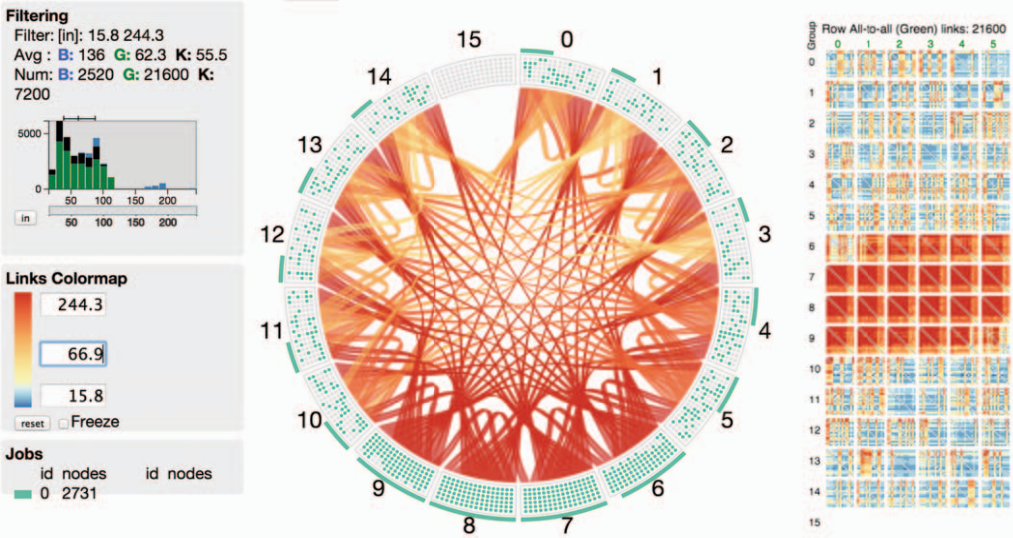
\includegraphics[width=0.8\textwidth]{dgfly_bhat}
%\centering
%\caption[Exemplo de rede \dgfly de três níveis com 64000 nós em execução, onde 2731 estão alocados para uma tarefa]{Exemplo de rede \dgfly de três níveis com 64000 nós em execução, onde 2731 estão alocados para uma tarefa. \Links globais apresentados no meio e links locais na matriz a direita. Quanto mais avermelhado, mais tráfego na rede~\cite{dragonfly}.}
%\label{fig:dgfly_bhat}
%\end{figure}

\subsection{Abstrações de Topologia}
\label{sec:abstrações}

Nesta seção são abordados dois trabalhos que abstraem informações de topologia para seu uso em aplicações: O \textit{Portable Hardware Locality} (\hwloc) \cite{broquedis:hwloc} e o \textit{Portable Network Locality}  (\netloc) \cite{Goglin:netloc}.

\Hwloc é um \textit{software} que provê uma abstração da hierarquia das arquiteturas de máquinas, dispondo uma série de informações de \textit{cache}, núcleos, \textit{multithreading}, \textit{sockets} e dispositivos de entrada e saída~\cite{broquedis:hwloc}.
Seu objetivo é facilitar o acesso de informações complexas das arquiteturas atuais, de maneira uniforme e portável para aplicações.
Em sistemas Unix, por exemplo, as informações coletadas por \hwloc estão em diversos arquivos espalhados pelo sistema. Portanto, diversas leituras de dados em disco são necessárias para adquirir estas informações.
Em questão de topologia, o \hwloc trabalha somente em um ambiente multiprocessado, em uma única máquina, não oferecendo suporte em relação a topologia de um ambiente multicomputado ou distribuído.

\Netloc~é um projeto de \textit{software} acoplado ao \hwloc que provê uma abstração da topologia de rede.
Assim como o \hwloc, o \textit{software} é usado para encontrar informações completas da topologia, ainda não descobertas, e disponibilizá-las para o usuário.
O trabalho do \netloc é voltado para métodos de descobrimento e representação da topologia de rede, unindo estas informações com as informações de máquina do \hwloc~\cite{Goglin:netloc}.

O projeto \netloc ainda está em desenvolvimento e ainda não possui representação de distância ou latência entre áreas distintas da rede.
Além disso, sua preocupação é de fornecer todas as informações que conseguir sobre a topologia utilizada de maneira dinâmica para considerar alterações na rede devido a falhas e expansões~\cite{Goglin:netloc}.
A quantidade e complexidade destas informações aumentam a ocupação de memória e o tempo de inicialização da abstração, adicionando um custo indesejado.

\section{Balanceamento de Carga}
\label{sec:lb}

Balanceamento de carga é uma técnica que realiza distribuição de cargas de computação e comunicação em um sistema de maneira que nenhum processador seja sobrecarregado e que reduza custos de comunicação~\cite{Becker}. 
Tendo em vista uma aplicação dinâmica, a distribuição de carga e comunicação se altera ao longo da aplicação, sendo necessário realizar um balanceamento de carga periodicamente para mitigar o desbalanceamento. 

Encontrar um mapeamento ótimo para uma aplicação paralela executada em múltiplas máquinas idênticas é um problema NP-\textit{hard}~\cite{leung}. 
Como o objetivo de balancear é aumentar o desempenho, utilizam-se heurísticas para realizar um balanceamento sub-ótimo, já que um mapeamento ótimo iria demorar a ponto de degradar o tempo da aplicação~\cite{pilla-thesis}.

Um balanceador de carga (\textit{Load Balancer} ou LB) pode administrar informações sobre a distribuição de carga e comunicação de três maneiras: \textit{centralizada}, \textit{distribuída} e \textit{hierárquica}.
Um LB centralizado administra a informação do sistema como um todo, podendo realizar decisões mais completas, mas criando um gargalo de informações. 
Um LB distribuído é o outro extremo pois observa somente informações locais, tendo um processo de balanceamento mais escalável, mais rápido porém menos efetivo. 
Uma abordagem hierárquica mistura as duas outras abordagens em camadas hierárquicas diferentes~\cite{Becker}.

Um balanceamento de carga pode utilizar informações da topologia da rede para posicionar tarefas que se comunicam próximas umas das outras, reduzindo a latência de comunicação e efeitos de contenção na rede.
Esta informação se torna ainda mais relevante quando o diâmetro de uma rede é grande, quando esta possui assimetria ou latências diferentes para partes diferentes da rede~\cite{dragonfly}.
Um LB que utiliza estas informações é dito ciente de topologia.

\subsection{Charm++}
\label{sec:charm}

\charm~\cite{website:CHARM} é um sistema de programação paralela independente de máquina desenvolvido na~\textit{University of Illinois at Urbana-Champaign}~\cite{Kale:charm}. 
O sistema é baseado na ideia de objetos migráveis chamado de \chares cuja execução é guiada pela troca de mensagens. 
O seu sistema de execução (\textit{runtime}) possibilita a execução de programas paralelos com mecanismos avançados, como balanceamento de carga automático e \textit{checkpointing}. 
\charm suporta tanto ambientes de multiprocessadores quanto de multicomputadores, conseguindo realizar comunicação através de memória compartilhada e de protocolos ou de infraestruturas de comunicação em rede, tais como UDP, MPI, OFI, Infiniband, uGNI e PAMI~\cite{pilla:CHARM}.

\Chares são objetos concorrentes utilizados no \fw \xspace \charm que possuem somente métodos de entrada visíveis, que são utilizados de maneira remota e assíncrona~\cite{Kale:charm}.
Com estes métodos, \chares podem se comunicar remotamente sem necessidade de barreiras. Pela sua natureza desacoplável, \chares são altamente migráveis, podendo trocar de PEs com facilidade. 

Para garantir a eficiência na troca de mensagens entre suas tarefas, a plataforma \charm adquire as informações de topologia da rede com o seu \textit{runtime}.
No início da execução de uma aplicação, é realizado uma troca de mensagens entre os processos em execução em busca de suas conexões.
Esta informação é utilizada para inferir a topologia utilizada dentre a seguinte lista: \textit{mesh}, \fatt, torus, anel e grafo completo. 


\section{Conclusão}
Em ambientes paralelos e distribuídos, informações da topologia podem ser utilizadas para melhorar o desempenho das aplicações.
Alocação de tarefas é uma das técnicas que se beneficia disto, podendo reduzir a latência de comunicação e a contenção de uma rede através de alocação próxima de tarefas que se comuniquem.
Estes fatores se tornam mais impactantes quando se considera redes indiretas e com custos de comunicação diferenciados entre partes da rede.

A plataforma \charm provê um ambiente para programação paralela com a possibilidade de utilização de balanceadores de carga. Porém, as informações topológicas adquiridas pela plataforma são imprecisas e apresentam limitações.
O próximo capítulo aborda a abstração proposta por este trabalho, Net Topo, que visa facilitar o acesso de algumas informações de topologia.


% ----------------------------------------------------------
% Parte de proposta do projeto
% ----------------------------------------------------------


% ---
% Capitulo de Proposta
% ---

\chapter{Net Topo}
\label{cap:proposta}

A contenção de rede e a latência de comunicação são dois fatores ligados à topologia de rede que afetam diretamente o desempenho de uma aplicação paralela e distribuída.
Estes dois fatores podem ser reduzidos com uma distribuição de carga que aloque tarefas que se comuniquem próximas uma da outra~\cite{bhatele-encyclopedia}.
Para saber o quão próximo um PE está de outro e realizar uma alocação eficiente, é preciso obter informações sobre a topologia da rede sendo utilizada.
Ferramentas para descobrimento e uso de informações de topologia existem, mas têm suas limitações.

A ferramenta \hwloc realiza o descobrimento e armazenamento de topologias de máquina, oferecendo um detalhamento profundo de qualquer informação da máquina, mas sem ter qualquer informação inter-máquina.
O projeto \netloc pretende estender o \hwloc adquirindo informações completas da camada de rede, porém está em desenvolvimento e, justamente por procurar um conjunto de informações grande, se torna caro em inicialização e em espaço de memória.
O \textit{runtime} \charm possui uma série de maneiras para utilizar uma topologia de rede, mas estas são enquadradas em alguns tipos de topologias pré-definidas, gerando algumas imprecisões.

Neste capítulo é abordado a Net Topo, uma abstração da topologia de rede criada neste trabalho que visa auxiliar escalonadores e balanceadores de carga cientes de topologia. 
Os objetivos da abstração são abordados na Seção~\ref{sec:net_objetivos}.
A Seção~\ref{sec:estruturas} apresenta as estruturas cogitadas e utilizadas na abstração.
Por último, as funcionalidades da abstração são descritas na Seção~\ref{sec:func}.

\section{Objetivos da Net Topo}
\label{sec:net_objetivos}

O principal objetivo da Net Topo é auxiliar na alocação e distribuição de carga fornecendo informações de uma topologia de rede.
Para que a abstração possa ser utilizada independente da topologia de um sistema, sua representação deve ser flexível e genérica, podendo comportar tipos diferentes de topologias sem perder funcionalidades.
Com isso, a abstração pode ser utilizada em escalonadores e balanceadores independentemente do sistema em que estejam.

O principal uso das informações de topologia para um escalonador ou balanceador de carga é indicar a proximidade entre tarefas, visando a redução de latência e contenção.
Para suprir esta informação, a abstração deve poder indicar a proximidade entre dois PEs na rede e suprir informações de distância como \hops ou latência.

Para acelerar o desenvolvimento e auxiliar escalonadores e balanceadores de carga, é importante que a abstração ofereça métodos úteis e não gere um sobrecusto que degrade o desempenho da aplicação.
Em outras palavras, a Net Topo não pode retardar demasiadamente o processo de distribuição de carga.

Um outro objetivo da abstração é oferecer persistência de informação entre execuções no mesmo sistema, seguindo a ideia do \hwloc de arquivar uma topologia. 
Esse arquivamento permite uma importação posterior das informações de topologia sem passar novamente por um processo de descobrimento, reduzindo o sobrecusto de inicialização da estrutura~\cite{broquedis:hwloc}.
Outro benefício é que o arquivo pode ser repassado para outras máquinas que tenham a mesma topologia de rede, para que não tenham que realizar o descobrimento da topologia.

A plataforma \charm oferece suporte para balanceadores de carga e oferece uma estrutura que facilita o desenvolvimento de um balanceador de carga. 
Um último objetivo da Net Topo é a integração com o módulo de balanceamento de carga do \charm.
Acoplar a abstração junto ao \charm aumenta a aplicabilidade da abstração e melhora o uso de uma plataforma já estabelecida.
 


    %\item Fornecer a distância e proximidade entre PEs dentro da rede e outras informações de topologia, para auxiliar tomadas de decisões em balanceadores e escalonadores.
    %\item Ser simples e com pouco sobrecusto, facilitando o desenvolvimento de balanceadores sem debilitar seu desempenho.
    %\item Arquivar uma topologia para uso futuro, para que uma topologia não tenha de ser descoberta ou inicializada novamente no mesmo sistema.
    %\item Fornecer suporte a plataforma \charm, para facilitar o desenvolvimento no módulo de balanceamento de carga.

\section{Estrutura}
\label{sec:estruturas}
% situando o que eh um grafo
% situando como pode ser mapeado um grafo pra topologia
Um grafo é uma maneira de representar informação como um conjunto de vértices e arestas que associam dois vértices.
Uma topologia de rede simétrica pode ser representada por um grafo não direcionado $G = (V, E)$ onde os vértices $V$ são PEs e as arestas $E$ são os \links entre PEs~\cite{Solihin}.
Para representar custo ou latência de um \textit{link}, é adicionado um peso $w$ a cada aresta $E$.
A forma de armazenamento das informações deste grafo influencia diretamente a forma de acesso aos dados e a quantidade de memória alocada no sistema.

% falar que há uma tabela com as estruturas propostas
Portanto, foram estudadas três abordagens de se armazenar as informações do grafo de topologia: (i) um armazenamento de todas as suas distâncias; (ii) um armazenamento do grafo de topologia; ou (iii) ambos.

O armazenamento de distâncias visa capturar somente a distância entre PEs, obtendo um acesso rápido e simplificado.
Para obter estas distâncias, necessita de um tempo maior de inicialização.
Esta opção gera menor ocupação de memória, pois armazena somente uma parcela sintetizada das informações.
Por outro lado, como não observa o agrupamento e a disposição da topologia, impedindo a utilização destas para distribuição de carga e em cálculos de proximidade.

A opção de armazenar o grafo visa manter as informações relevantes para distribuição de carga, mantendo a possibilidade de obter distâncias.
Quando comparada com a opção de armazenar somente distância, ocupa mais memória e é mais lenta no acesso de distâncias, precisando iterar sobre a estrutura para as obter.
Para acelerar a obtenção destas distâncias é possível utilizar mecanismos de programação dinâmica, como uma \textit{cache}, para manter uma parcela das distâncias calculadas. 

A opção de guardar tanto as distâncias calculadas quando a estrutura geral de topologia gera uma ocupação de memória agregada mas obtém os benefícios de ambas.
Esta opção foi a escolhida para este trabalho.
Ela permite utilizar as informações da topologia, realizar um cálculo de distâncias rápido e não impede extensões futuras.
A penalidade desta opção é uma utilização maior de memória.
O armazenamento completo das distâncias em vez de uma \textit{cache} é devido a persistência de informações entre execuções, onde a \textit{cache} não necessariamente manteria localidade devido a padrões diferentes de comunicação e distribuição.

Existem diversas estruturas de dados para armazenar as informações de um grafo, e seus benefícios são dependentes de como esta estrutura é utilizada.
O grafo de topologia sendo armazenado é dado por $G = (V, E, W)$, onde $V = \{$ união dos $v \in V$, que representam PEs$\}$, $E = \{$ união das relações $(v, u) \mid v, u \in V\}$, $W$ é uma função de peso $W:v,u \rightarrow \mathbb{R}$.
Foram avaliadas quatro estruturas de dados para o armazenamento de $G$, observando suas vantagens, desvantagens e aplicabilidade para este projeto. Elas são descritas a seguir.

\begin{itemize}
    \item \textbf{Lista de listas}: Uma representação que dispõe $V$ em uma lista $L$ e para cada $v \in V$ há uma lista de arestas $L_v \mid \forall e \in E, e \in L_v \iff v \in e$. 
    É uma estrutura simples que tem tempo de acesso de $O(\mid L_v \mid$).
    Ocupa memória em complexidade $O(\mid V \mid \times \mid L_v \mid)$.
    Esta estrutura é utilizada no \fw de balanceamento de carga do \charm.

    \item \textbf{Árvore}: Uma árvore representando uma hierarquia de proximidade. 
    Tem tempo de acesso de $O(log_f \mid V \mid)$ e ocupa memória relativa a $O(\mid V \mid)$.
    A base do logaritmo $f$ depende do número de divisões por camada da árvore (chamado de \textit{fanout}).
    É utilizada no \hwloc para a estrutura topológica interna de uma máquina. 
    No \hwloc os PEs se encontram como folhas da árvore e são agrupados de acordo com a proximidade dentro da máquina.
    Esta abordagem se adéqua bem para topologia interna devido a sua hierarquia inerente, mas não descreve bem uma topologia não hierárquica, como uma torus, pois muitas máquinas se encontram no mesmo nível hierárquico, possuem arestas entre si e não necessariamente contém uma hierarquia com mesmo \textit{fanout} ou profundidade.
    Uma árvore não tem inserção de ligação.
    
    \item \textbf{Matriz}: Uma matriz representando todas as associações possíveis entre os PEs da rede.
    Tem tempo constante de acesso a uma ligação mas ocupa memória quadrática em relação a $\mid V \mid$.
    Uma das vantagens de uma matriz é sua alta mutabilidade de ligações, sendo possível alteração ou inserção posteriores de ligações na topologia com tempo constante.

    \item \textbf{\textit{Compressed Sparse Columns}} (CSC): uma representação construída a partir de uma matriz, retirando todas as ligações inexistentes para economia de memória.
    A estrutura é organizada em três listas: uma lista com os valores não nulos da matriz, uma lista com as linhas destes valores e uma lista que indexa o início das linhas de cada coluna.
    Utiliza índices de acesso similar a uma lista de listas.
    É feita de maneira a otimizar localidade temporal de memoria quando é realizado uma travessia do grafo.
    Um CSC também pode ser distribuído de maneira reduzida, sem prejudicar um algoritmo de travessia de grafos~\cite{sun:csr}.
    O problema de uma CSC é sua baixa mutabilidade, necessitando uma refatoração para inserir novas arestas ou de um número de espaços vazios na sua inicialização, que podem não ser o suficiente.
\end{itemize}

Na Tabela~\ref{tab:struct_comparison} é observada a complexidade do tempo de leitura de uma ligação específica da estrutura, de tamanho ocupado na memória e de inserção de uma ligação, todos em relação ao número de vértices $p = \mid V \mid$, ao número de arestas $l = \mid E \mid$ e ao grau $g$ da topologia. 

\setlength{\tabcolsep}{0.5em}
\begin{table}[t]
    \centering
    \begin{tabular}{l c c c}
        \toprule
        \textbf{Estrutura} & \textbf{Leitura} &  \textbf{Memória utilizada} & \textbf{Inserção de ligação} \\ \midrule
        %\hline
        Listas de Listas & $O(g)$ & $O(p \times g)$ & $O(2g)$ \\
        Matriz & $O(1)$ & $O(p^2)$ & $O(1)$ \\
        Árvore & $O(log_f p)$ & $O(p)$ & $*$ \\
        CSC &  $O(g)$ & $O(p+l)$ & $O(p + l)$  \\ \bottomrule
    \end{tabular}
    \caption[Complexidade de leitura e de memória das estruturas cogitadas.]{Complexidade de leitura e de memória das estruturas cogitadas em relação ao número de vértices $p = \mid V \mid$, ao número de arestas $l = \mid E \mid$ e ao grau $g$ da topologia. A estrutura de Árvore depende também de um fator de \textit{fanout} $f$. }
    \label{tab:struct_comparison}
\end{table}

Uma estrutura puramente topológica não proveria um acesso rápido para distância, pois teria de calculá-la a cada chamada.
Para acelerar o acesso às distâncias, pode-se usar uma técnica de programação dinâmica denominada \textit{memoização}.
A técnica consiste em armazenar uma informação indireta em uma estrutura, para que não tenha que ser calculada novamente.
Uma estrutura somente de distâncias, se usada como um mecanismo de memoização, iria ser ampliada até que em algum momento conteria todas as distâncias possíveis, onde $g = p$ e $p = l^2$. 
Quando isto ocorrer, todas as estruturas apresentadas ocupariam memória quadrática em relação a $p$, exceto uma árvore, que não oferece um acesso constante à distância.
Dentre as estruturas de dados apresentadas, a matriz é a com acesso mais rápido neste caso, sendo a estrutura candidata para memoização completa.
Esta abordagem não escalaria com o número de PEs. Realizar uma abordagem com ambas as estruturas resultaria num uso extenso da memória, algo indesejável para uma aplicação distribuída e escalável.

Para alcançar escalabilidade, foi utilizada uma estrutura inspirada no \netloc, dividindo a topologia em dois níveis: uma camada hierárquica em árvore que representa a topologia interna das máquinas, similar ao \hwloc, e outra camada que apresenta as conexões em um nível de rede, representada com CSC pela sua utilidade em travessia de grafos. 
Uma matriz de distâncias foi utilizada como mecanismo de memoização para distâncias no nível de rede, reduzindo seu tamanho por considerar somente um nível de hierarquia. 
Além disto, foi assumido simetria no nível de rede, possibilitando a compressão desta matriz para uma matriz triangular superior.
A utilização desta matriz é opcional e pode ser removida.

\begin{figure}[t]
\begin{subfigure}{.5\textwidth}
    \centering
    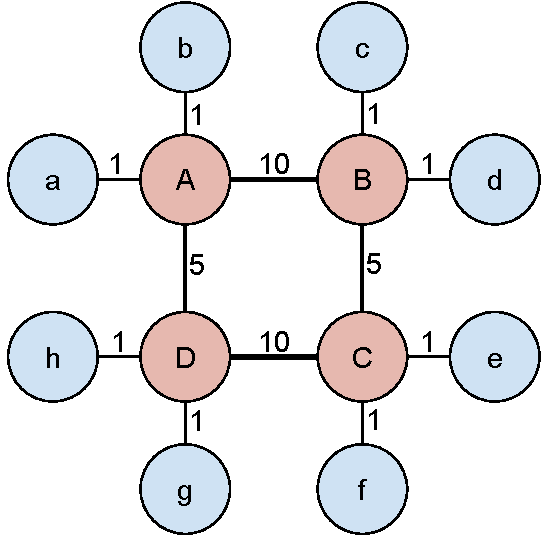
\includegraphics[width=0.8\linewidth]{images/estrutura_abst_topo.pdf}
    \caption{Topologia.}
    \label{fig:estru:topo}
\end{subfigure}
\begin{subfigure}{.5\textwidth}
    \centering
    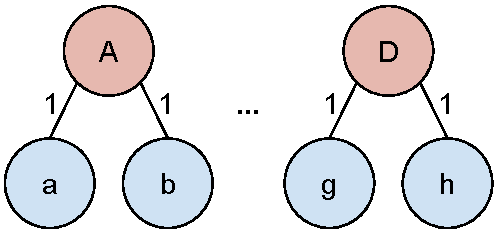
\includegraphics[width=0.8\linewidth]{images/estrutura_abst_arvore.pdf}
    \caption{Árvore.}
    \label{fig:estru:arvore}
\end{subfigure}
\begin{subfigure}{.5\textwidth}
    \centering
    \begin{tabular}{|l|c|c|c|c|c|c|c|c|}
        \cline{1-6}
        Índice     & 0 & 2  & 4 & 6 & 8  \\ \hline
        Linha      & B & D & A & C & B & D & A & C  \\ \hline
        Distância  & 10 & 5 & 10 & 5 & 5 & 10 & 5 & 10 \\ \hline
    \end{tabular}
    \caption{CSC.}
    \label{fig:estru:csc}
\end{subfigure}
\begin{subfigure}{.5\textwidth}
    \centering
    \begin{tabular}{|c|c|c|c|c|}
        \hline
         M & A & B  & C & D  \\ \hline
         A & X & 10 &   & 5  \\ \hline
         B & X & X  & 5 & 15 \\ \hline
         C & X & X  & X & 10  \\ \hline
         D & X & X  & X & X  \\ \hline
    \end{tabular}
    \caption{Matriz.}
    \label{fig:estru:matriz}
\end{subfigure}
\caption[Representação das estruturas utilizadas.]{Representação da topologia mostrada em (a)-(b) de acordo com as estruturas propostas.}
\label{fig:estru}
\end{figure}

A Figura~\ref{fig:estru} apresenta as estruturas propostas para representar a topologia da Figura~\ref{fig:estru:topo}, os PEs então em azul, as máquinas em vermelho e os números nas conexões representam uma latência. 
A Figura~\ref{fig:estru:arvore} apresenta a estrutura hierárquica de árvore de duas das máquinas desta topologia e a Tabela~\ref{fig:estru:csc} a representação das distâncias das máquinas com CSC. 
A estrutura matricial para memoização das distâncias entre máquinas é representada pela Tabela~\ref{fig:estru:matriz}. Ela utiliza uma estrutura matricial proposta para a memoização de distâncias entre as máquinas, onde a primeira linha e primeira coluna indicam uma máquina e as células internas representam as distâncias.
Um 'X' indica que a posição não é armazenada para economia de memória e um espaço em branco indica uma distância ainda não calculada mas com memória alocada.

Nesta estrutura, a complexidade de acesso de uma distância qualquer é de $O(g)$ e de $O(1)$ caso tenha sido calculada anteriormente.
Sendo $c$ a média do número de PEs por máquinas e $m$ o número de máquinas, o uso de memória é de $O(mc)$ para as estruturas de árvore, de $O(\frac{p+l}{c})$ para o CSC e de $O(\frac{p^2}{2c^2})$ para a matriz de memoização.
O custo de criação e inicialização da estrutura é dependente do número de PEs na rede e do tempo de acesso e descobrimento das informações topológicas usadas de base, como a do \hwloc ou do \textit{runtime} \charm.



\section{Funcionalidades}
\label{sec:func}

A interface da Net Topo contém métodos para obter informações da topologia, cálculo de distância, \hops e proximidade, abordados na Seção~\ref{sec:distances}, e para a serialização das estruturas em um arquivo XML, descrito na Seção~\ref{sec:xml}.
Na Seção~\ref{sec:init} é detalhado como são inicializadas as estruturas da abstração.
A Tabela~\ref{tab:topo_infos} apresenta as informações de topologia disponíveis na abstração, seus métodos e suas assinaturas.
A palavra ``nó'' é utilizada para representar um agrupamento interno de PEs de uma máquina, realizado por nível de \textit{cache} compartilhada.

\setlength{\tabcolsep}{0.5em}
\begin{table}[t]
    \centering
    \begin{tabular}{l c l}
        \toprule
        \textbf{Método} &    \textbf{Entrada} &    \textbf{Saída} \\ \midrule
        \textit{num\_pes} &    - &    Número de PEs na topologia   \\ 
        \textit{num\_machines} &    - &    Número de máquinas na topologia   \\
        \textit{num\_nodes} &    - &    Número de nós na topologia   \\
        \textit{machine\_of} & um PE & Máquina onde o PE se encontra  \\
        \textit{node\_of} & um PE & Nó onde o PE se encontra  \\
        \textit{pes\_of\_machine} &  uma máquina & Uma lista dos PEs da máquina \\
        \textit{on\_same\_machine} &  uma PE & Uma lista dos PEs na mesma máquina \\
        \textit{pes\_of\_node} &  um nó & Uma lista dos PEs do nó \\
        \textit{on\_same\_node} &  uma PE & Uma lista dos PEs no mesmo nó \\
        \textit{net\_neighbors} &  uma máquina & Uma lista de máquinas vizinhas \\ \textit{num\_net\_links} & - & Número de \textit{links} na rede \\
        \textit{fill\_memoi} & - & Preenche a matriz de memoização \\
        \bottomrule
    \end{tabular}
    \caption[Métodos de informação de topologia.]{Métodos de informação de topologia. A primeira coluna apresenta a assinatura do método. A coluna Entrada apresenta as informações requeridas pelo método e a coluna Saída indica o que o método retorna.}
    \label{tab:topo_infos}
\end{table}

\subsection{Funções de Distância e Proximidade}
\label{sec:distances}

Métricas de proximidade entre dois PEs e a distância entre eles são relevantes para realizar uma alocação de tarefas eficiente e que leve em consideração a topologia de rede utilizada.
Três métricas de distância foram implementadas dentro da Net Topo: uma função de proximidade, um cálculo de \hops e um cálculo de distância mínima.

Como os custos de comunicação aumentam conforme a distância entre PEs, saber em que nível a comunicação irá acontecer permite uma estimativa do custo de comunicação entre dois PEs.
Para determinar qual a camada de comunicação entre dois PEs, basta saber da topologia de máquina de uma delas. 
Se não estiverem na mesma máquina, esta acontecerá em rede. 
Se estiverem, é possível determinar em qual nível.
A função de proximidade realiza um cálculo simples para indicar o quão próximo um PE está de outro na topologia de máquina.
O método que implementa esta função tem o nome de \textit{proximity}, recebe dois identificadores de PE como entrada e retorna um inteiro de acordo com a função de proximidade descrita na Tabela~\ref{tab:proximity}.
Saber o quão próximo um ponto está de outro em uma rede é dependente ou de sua distância mínima ou da quantidade de \hops até ele, que caem no escopo das próximas funções e não são tão simples.


% tabelinha de retorno de função de proximidade
\setlength{\tabcolsep}{0.5em}
\begin{table}[!ht]
    \centering
    \begin{tabular}{c l}
        \toprule
        \textbf{Saída} &    \textbf{Relação entre os dois PEs} \\ \midrule
        3 & São o mesmo.   \\ %\hline
        2 & Estão na mesma máquina e no mesmo nó.   \\ %\hline
        1 & Estão na mesma máquina mas não no mesmo nó.   \\ %\hline
        0 & Não estão na mesma máquina. \\ \bottomrule
    \end{tabular}
    \caption[Função de proximidade]{Função de proximidade entre dois PEs. A primeira coluna representa a saída da função e a segunda a relação entre os dois PEs.}
    \label{tab:proximity}
\end{table}

Um cálculo de \hops permite observar a proximidade entre dois PEs em uma rede, a quantidade de \links utilizada em uma comunicação entre os dois e ter uma noção de distância sem precisar obter as latências da rede.
O cálculo de \hops é implementado pelo método \textit{hop\_count}, que recebe identificadores de dois PEs, um origem e um destino, e retorna um inteiro com o número de \hops.
A implementação é uma busca em largura pela estrutura CSC, iniciando no PE origem e contando o número de expansões até alcançar o PE destino.
Esta implementação não utiliza o mecanismo de memoização, pois as distâncias mínimas são diferentes do número de \hops.


Um cálculo de latência mínima entre dois PEs permite considerar com precisão a latência de comunicação entre eles mas não oferece uma perspectiva de contenção.
Essa informação é útil para um escalonador ou balanceador que visa reduzir as latências de comunicação do sistema.

O cálculo de distância mínima foi implementando utilizando o algoritmo de Djisktra modificado para incluir o mecanismo de memoização.
Antes de ser executado na camada de rede, é obtida a máquina dos dois PEs e é verificado se são os mesmos. Caso sejam, é retornado $0.1$ se estão no mesmo nó, $0$ se são o mesmo PE e $0.2$ caso nenhum dos dois seja verdade.

O Algoritmo~\ref{alg:dists} apresenta o algoritmo modificado.
$M$ é uma função cujo domínio são dois PEs da topologia, $x$ e $y$, e a imagem é a distância entre eles seguindo uma matriz de distâncias. %ref equação
%A função $M$ é uma função de mapeamento $M:x,y \rightarrow \mathbb{Z} \mid x, y \in \mathbb{Z}$, onde $x$ e $y$ representem máquinas e o valor retornado representa a distância entre eles.
A função representa o mecanismo de memoização implementado com uma matriz triangular superior.
Para inserir um valor na posição $(x, y)$ da matriz de distâncias de $M$, se utiliza a notação $M[x][y] \leftarrow$ distância.
O mapeamento $D:m \rightarrow d$ associa uma máquina $m$ a uma distância $d$ da origem.
A notação $D(m) \rightarrow d$ é utilizada para indicar que uma nova associação foi criada.

No inicio do Algoritmo~\ref{alg:dists} é verificado se a distância entre a origem e o destino já não é conhecida na estrutura de memoização.
Caso seja, a distância é retornada e o algoritmo encerra.
Nas linhas 1 a 10 ocorre a inicialização do algoritmo, adicionando máquinas cuja distância já se sabe ao conjunto das não visitadas. 
Nas linhas 11 a 27 é executado o laço principal, onde, para cada máquina do conjunto de máquinas não visitadas ($U$), se alcança suas vizinhas e, caso não tenham sido alcançadas, as adiciona em $U$.
Caso a máquina vizinha tenha sido alcançada, é verificado se a distância atual até ela não é menor do que a armazenada no momento (linha 18).
Antes de trocar a máquina sendo visitada (linhas 20 a 22), se insere sua distância em $M$ para uso futuro, a adiciona ao conjunto das visitadas ($V$) e a retira de $U$.
Ao se trocar de máquina (linha 23) é sempre escolhida a máquina menos distante de $U$ e, caso seja o destino, sua distância é adicionada em $M$ e o algoritmo termina retornando a distância encontrada.
Caso não se alcance o destino, é retornado $-1$.

\begin{algorithm}[t]
\caption{Djisktra Modificado}
\label{alg:dists}
    \DontPrintSemicolon
    \SetKwInOut{Estrutura} {Estruturas}
    \Entrada{origem: máquina de origem, destino: máquina destino}
    \Saida{Distância entre a origem e o destino}
    \Estrutura{$V$: Conjunto de máquinas visitadas, \\ 
                $U$: Conjunto de máquinas não visitadas, \\
                $D$: Mapeamento de uma máquina para uma distância.}
                \BlankLine
    $U \leftarrow \{$origem$\}$\;
    $D($origem$) \leftarrow {0}$\;
     \ForEach{máquina "x" da topologia}{
        $U \leftarrow U \cup \{x\}$\;
        \eIf{$M[$origem$][x]$ existe}
            {$D(x) \rightarrow M[$origem$][x]$}
        {$D(x) \rightarrow \infty$}
    }
    atual $\leftarrow$ origem  \tcp*{máquina sendo iterada}
    dist $\leftarrow 0$  \tcp*{distância até o atual}
    \While{$U \neq $\O}{
        \ForEach{máquina "v" $\mid$ v é vizinha da máquina atual}{
            $dist\_v \leftarrow$ dist $+$ distância entre atual e $v$\;
            \eIf{$v \notin \{V \cup U\} $}{
                $U \leftarrow U \cup \{v\}$\;
                $D(v) \rightarrow dist\_v$}
                {\If{$v \in U$ e $D(v) > dist\_v$}
                    {$D(v) \rightarrow dist\_v$}
            }
        }
        $M[$origem$][$ atual$] \leftarrow$ dist\;
        $V \leftarrow V \cup \{$atual$\}$\;
        $U \leftarrow U \setminus \{$atual$\}$\;
        atual $\leftarrow x \mid x \in U$ e tenha a menor distância em $U$\;
        dist $\leftarrow D($atual$)$\;
        \If{atual = destino}{
            $M[$origem$][$ destino$] \leftarrow$ dist\;
            retorna dist}
    }
    retorna $-1$ \tcp*{não alcançou o destino}
\end{algorithm}

Foi cogitado a importação das distâncias memoizadas de uma máquina vizinha na linha 12 com um laço adicional, mas geraria um sobrecusto que não seria sempre útil.
A utilização dela não é sempre melhor devido ao fato de que a distância memoizada é relativa à distância de alcançar a máquina sendo visitada, portanto não necessariamente será o menor até o alvo, mas somente a menor a partir do atual.


\subsection{Serialização}
\label{sec:xml}

O armazenamento da estrutura de topologia permite utilizar a mesma estrutura topológica em execuções diferentes, reduzindo o custo de inicialização da abstração e mantendo persistência das informações de custos já calculadas.

Para realizar a serialização das estruturas da Net Topo, foi utilizado a biblioteca de serialização \textit{Cereal} ~\cite{website:Cereal}. 
A biblioteca foi escolhida pela sua simplicidade, velocidade e pela compatibilidade com a linguagem \textit{C++}.
O arquivo de serialização gerado está na linguagem XML (\textit{Extensible Markup Language}), o mesmo utilizada pelo \hwloc, pois oferece legibilidade do que está armazenado.

Foram criadas as funções \textit{save\_topology} e \textit{load\_topology} para exportar e importar, respectivamente, um arquivo XML com nome passado por parâmetro.
Caso nenhum nome seja passado, o nome padrão utilizado é ``\textit{net\_topo.xml}''.
Para inicializar as estruturas com as informações armazenadas num arquivo, basta chamar a função \textit{load\_topology} após a criação de uma instância da Net Topo.


\subsection{Inicialização}
\label{sec:init}

Para ampliar e facilitar seu uso, a Net topo é uma abstração desacoplada de outras implementações, o que faz que sua inicialização seja dependente de alguma fonte de informações topológicas.
As informações de rede podem ser obtidas manualmente ou através de mecanismos automáticos, como o \netloc.
O \textit{runtime} \charm obtém informações de topologia automaticamente.
A Seção~\ref{sec:init:charm} apresenta detalhes das informações obtidas pelo \charm e como estas informações são passadas para a abstração.

Neste trabalho foram criadas três inicializações: uma manual, que recebe uma entrada padrão; uma automática, utilizando um adaptador para o \charm; e uma através de um arquivo XML gerado anteriormente pelo Net Topo.
As três formas de inicialização são abordadas a seguir e todas têm a opção de remover o mecanismo de memoização.

\subsubsection{Inicialização Manual}

Um padrão de entrada com as informações de topologia necessárias foi criado para a função de inicialização do Net Topo.
O algoritmo de funcionamento da inicialização da estrutura foi dividido em dois e é descrito pelos Algoritmos~\ref{alg:init_machine} e \ref{alg:init_network}. 


A inicialização da topologia de máquina é descrita pelo Algoritmo~\ref{alg:init_machine} e deve ser executada antes, por capturar informações necessárias para a divisão de rede.
O objetivo deste algoritmo é criar um mapeamento entre PEs, nós e máquinas, para a representação da topologia de máquina.
O algoritmo necessita como entrada um conjunto de triplas $(pe, m, n) \mid pe, m, n \in \mathbb{Z}$ onde $pe$ representa um PE, $m$ representa a máquina deste PE e $n$ o seu nó. 
Os nós recebidos na entrada são relativos a uma máquina e não ao sistema como um todo.
O algoritmo assume que todos os PEs de uma máquina estejam em sequência nesta lista.
O resultado deste algoritmo são duas listas de duplas $PM$ e $PN$, um agrupamento de PEs por nó e um agrupamento de PEs por máquina.
O mapeamento $MP:m\rightarrow P$ associa um conjunto de PEs $P$ a máquina $m$.
Para associar o conjunto $P$ a uma máquina $m$ no mapeamento $MP$, é usada a notação $MP(m) \rightarrow P$.
O mapeamento $NP:n\rightarrow P$ associa um conjunto de PEs $P$ a um nó $n$.
Para adicionar um PE $pe$ ao conjunto $P$ de um nó $n$, é utilizado a notação $NP(m) \rightarrow pe$.
A notação $\mid NP \mid$ é utilizada para indicar o número de mapeamentos em $NP$.

\begin{algorithm}[t]
    \DontPrintSemicolon
    \SetKwInOut{Estrutura}{Estruturas}
    \Entrada{$T$: Conjunto ordenado de triplas $(m, pe, n)$, onde $m$ é uma máquina, $pe$ um PE desta máquina e $n$ o nó deste PE.}
    \Saida{ $PM$: Conjunto de duplas $(pe, m)$ onde $pe$ é um PE e $m$ sua máquina, \\
            \hspace{12mm} $PN$: Conjunto de duplas $(pe, n)$ onde $pe$ é um PE e $n$ seu nó, \\
            \hspace{12mm} $MP$: Mapeamento de cada máquina ao seu conjunto de PEs, \\
            \hspace{12mm} $NP$: Mapeamento de cada nó aos seus PEs.}
    \Estrutura{$P$: Conjunto de PEs de uma máquina.}

    \BlankLine
    $maq \leftarrow 0$, \xspace 
    $no \leftarrow 0$ \tcp*{máquina e nó sendo iterados}
    $n\_nos \leftarrow 0$\;
    $P \leftarrow $\O, \xspace
    $PM \leftarrow $\O, \xspace
    $PN \leftarrow $\O\;
    \ForEach{ tripla (m, pe, n) em T}{
        $PM \leftarrow PM \cup \{(pe, m)\}$\;
        \If{m $\neq$ maq}{
            $MP(maq) \rightarrow P$\;
            $maq \leftarrow m$\;
            $n\_nos \leftarrow \mid NP \mid$ \;
            $P \leftarrow $\O\;
        }
        $no \leftarrow n + n\_nos$\;
        $PN \leftarrow PN \cup \{(pe, no)\}$\; 
        $NP(no) \rightarrow pe$\;
        $P \leftarrow P \cup \{pe\}$\;
    }
    $MP(maq) \rightarrow P$\;
    
\caption{Inicialização da Topologia de Máquina}
\label{alg:init_machine}
\end{algorithm}

Nas linhas 1 e 3 do Algoritmo~\ref{alg:init_machine} são feitos os ajustes iniciais para a execução. 
O laço principal (linhas 4 a 15) mapeia cada PE para a sua máquina e para o seu nó (com os conjuntos $PM$ e $PN$). 
Cada máquina e cada nó é associado a um conjunto de PEs com os mapeamentos $MP$ e $NP$, respectivamente.
Na linha 11 é re-identificado o nó do PE, para ser absoluto e não relativo à máquina que estava.
Quando se troca a máquina sendo iterada (linhas 6 a 10) são agrupados para a máquina todos os PEs em $P$ para utilizar no mapeamento $MP$.
Na troca de máquina também é atualizada a contagem de nós encontrados até o momento, para modificar o número de identificação dos nós.



\begin{algorithm}[t]
    \DontPrintSemicolon
    \SetKwInOut{Estrutura}{Estruturas}
    \Entrada{$T$: um conjunto de triplas $(pe, v, d)$, onde $pe$ e $v$ são PEs vizinhos e $d$ a distância entre eles.}
    \Saida{$G$: um grafo de máquinas que representa a topologia de rede.}
    \Estrutura{
                $D$: conjunto de duplas \{$v, d$\}, onde $v$ é uma máquina e $d$ uma distância.
    }
    \BlankLine
    $V \leftarrow$ \O, \xspace
    $E \leftarrow$ \O\;
    \ForEach{máquina m na topologia}
        {$D \leftarrow vizinhas(m, T)$\;
        $V \leftarrow V \cup \{m\}$\;
        \ForEach{ dupla (v, d) em D} 
            {$V \leftarrow V \cup \{v\}$ \;
             $E \leftarrow E \cup \{(m, v)\}$\;
             $W(m, v) \rightarrow d$}
    }

\caption{Inicialização da Topologia de Rede}
\label{alg:init_network}
\end{algorithm}

O algoritmo de inicialização de topologia de rede, Algoritmo~\ref{alg:init_network}, captura as informações de vizinhança descrita por uma entrada ($T$), estabelece as vizinhanças em nível de máquina e as armazena em um grafo $G$.
O grafo $G$ é um grafo representando uma topologia de rede e é dado por $G = (V, E, W) \mid V = \{$ união dos $v$, que representa máquinas$\}$, $E = \{$ união das relações $(v, u) \mid v, u \in V\}$, $W$ é uma função de peso $W:v,u \rightarrow w$.
Este grafo é implementado com um CSC.
A função $vizinhas$ utilizada é descrita pelo Algoritmo~\ref{alg:vizinhos} e encontra as máquinas vizinhas de uma determinada máquina e suas distâncias até ela.

O algoritmo de inicialização da topologia de rede busca todas as máquinas vizinhas de cada máquina na topologia (linha 3).
Esta máquina é adicionada ao grafo como um vértice (linha 4) e para cada máquina vizinha é criado uma aresta com peso equivalente a distância até ela (linhas 7 e 8).

\begin{algorithm}
    \DontPrintSemicolon
    \SetKwInOut{Estrutura}{Estruturas}
    \Entrada{$T$: um conjunto de triplas $(pe, v, d)$, onde $pe$ e $v$ são PEs vizinhos e $d$ a distância entre eles, \\
            \hspace{15mm} $m$: uma máquina cuja vizinhança se quer conhecer.}
    \Saida{$V$: conjunto de duplas \{$v, d$\}, onde $v$ é uma máquina vizinha a $m$ e $d$ a distância entre elas.
                }
    \BlankLine
    
    $maq\_v \leftarrow 0$\; 
    $V \leftarrow $\O\;
    \ForEach{ tripla (pe, v, d) em T $\mid$ maquina\_de(pe) = m}{
        $maq\_v \leftarrow maquina\_de(v)$\;
        \eIf{maq\_v $\notin$ V}
            {$V \leftarrow V \cup \{maq\_v, d\}$}
            {\If{$V(maq\_v) > d$}
                {$V(maq\_v) \leftarrow d$}
        }
    }
    $V \leftarrow V \setminus \{m\}$\;
\caption{Máquinas Vizinhas}
\label{alg:vizinhos}
\end{algorithm}

O Algoritmo~\ref{alg:vizinhos} estabelece um conjunto das máquinas vizinhas de $m$ e a distância entre elas.
A funcionalidade $maquina\_de(pe)$ retorna a máquina de um PE $pe$.
O laço principal do algoritmo obtém todos os vizinhos de cada PE da máquina, criando duplas de máquinas vizinhas com as suas distâncias, agregadas no conjunto $V$.
Como cada máquina tem vizinhança consigo mesma, é necessário retirar ela mesma do mapeamento (linha 10).
Para obter a distância de uma máquina a outra, a menor distância dentre os PEs é utilizada, assumindo que uma latência entre PEs da mesma máquina possa ser desconsiderada no cálculo.

\subsubsection{Inicialização via XML}

A inicialização XML importa informações salvas anteriormente em um arquivo XML, restaurando a topologia armazenada e sua matriz de distâncias.
Para utilizar esta inicialização basta invocar o método \textit{load\_topology}, descrito na Seção ~\ref{sec:xml}.
A utilidade desta inicialização se dá pela remoção do tempo de descobrimento da topologia e pela importação da matriz de distâncias utilizada em execuções anteriores.
Esta inicialização só pode ocorrer se houver um arquivo XML de topologia salvo anteriormente.

% ver diferença de importação e descobrimento em testes de overhead?

\subsubsection{\charm}
\label{sec:init:charm}
A inicialização através do \textit{runtime} do \charm é automática mas apresenta uma série de limitações devido a incompletude das informações coletadas pelo \textit{runtime} e pelo armazenamento destas, abordadas adiante.

O \charm possui duas maneiras de descobrir uma topologia: de maneira manual, com opções de execução, da classe \textit{TopoManager} e topologias fixas como \textit{Cray} e \textit{BlueGene}; e de maneira automática, através de envio de mensagens entre os PEs utilizados e enquadramento da topologia encontrada em um dos tipos pré-estabelecidos em sua classe \textit{topology}, como \textit{Mesh} 2D, \textit{Torus} ou \Fatt. 
A escolha destas abordagens se deve a otimizar o calculo de \hops, que depende só das posições da origem e do destino nestas topologias, evitando um algoritmo com travessia de grafo.
Porém, os únicos métodos obrigatórios em cada topologia são os de encontrar o número máximo de vizinhos e os seus vizinhos, o que acarreta em dificuldades para algoritmos que consideram topologias genéricas.

A obtenção de topologia do \charm inclui três problemas que não eram esperadas no inicio deste trabalho:
(i) não há armazenamento de latência de mensagens entre PEs reconhecidos na topologia; (ii) não há informações sobre compartilhamento de \textit{cache} entre PEs; e (iii) há imprecisões em certas funções quando as máquinas da rede não são iguais.
A ausência de latências impossibilita cálculos de distância que não sejam através de \hops, pois não há nenhuma outra métrica.
A falta de informações sobre compartilhamento de \textit{cache} impede o agrupamento de PEs por grupos de \textit{cache} e um detalhamento de cada máquina na topologia.
As funções imprecisas são relacionadas ao número de PEs por nó físico da topologia, que são distribuídos igualmente pelo número de máquinas na rede.
Esse agrupamento equivalente impossibilita saber quais PEs estão efetivamente em quais máquinas, gerando informações imprecisas para a secção entre topologia das máquinas e topologia da rede.

A Figura~\ref{fig:charm_imprecision} apresenta uma comparação entre uma topologia real com máquinas heterogêneas e a sua representação dentro do sistema do \charm. A topologia é composta por duas máquinas, uma com 4 cores, sem agrupamento de \textit{cache}, e a segunda com 8 cores e 4 agrupamentos de \textit{cache}.

\begin{figure}[h]
\begin{subfigure}{.55\textwidth}
    \centering
    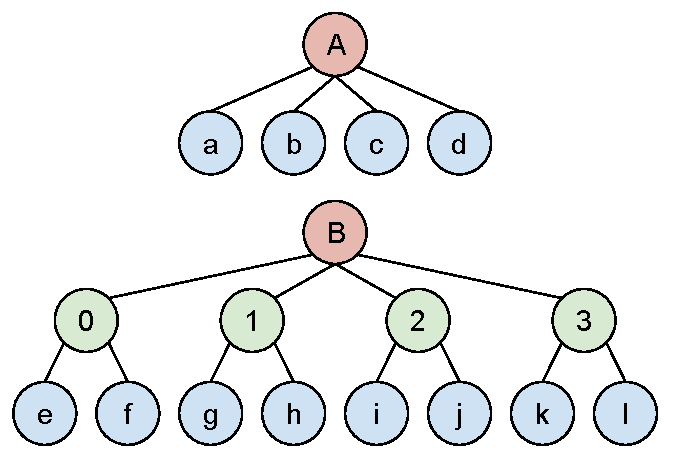
\includegraphics[width=0.85\linewidth]{images/init_real_topo.pdf}
    \caption{Topologia Real}
    \label{fig:charm_imprecision:real}
\end{subfigure}
\begin{subfigure}{.45\textwidth}
    \centering
    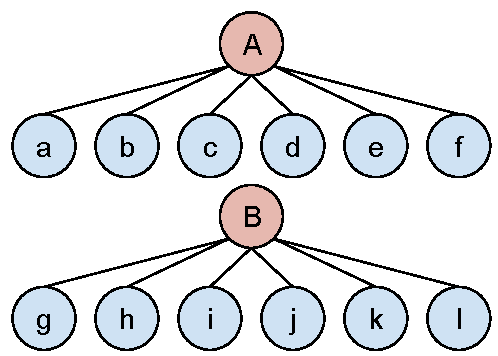
\includegraphics[width=0.8\linewidth]{images/init_charm_topo.pdf}
    \caption{Agrupamento realizado pelo \charm}
    \label{fig:charm_imprecision:charm}
\end{subfigure}
\caption[Comparação entre a topologia real e a encontrada pelo \charm.]{Comparação entre a topologia real (esquerda) e a encontrada pelo \charm (direita). Máquinas em vermelho e letras maiúsculas, agrupamentos de \textit{cache} em verde e numerais, e PEs em azul e letras minúsculas.}
\label{fig:charm_imprecision}
\end{figure}

Para interagir com o \textit{runtime} do \charm e extrair as informações topológicas foi criado um adaptador de nome \textit{net\_topo\_charm\_proxy}.
Dentro do adaptador foram criados duas inicializações intermediárias: \textit{init} e \textit{init\_no\_nodes}.
O primeiro extrai os agrupamentos de máquinas enquanto o segundo ignora a parte de topologia de máquina do \charm e trata cada PE como uma máquina individual.
Portanto, o segundo mantém a precisão das conexões mas perde qualquer informação relacionada ao agrupamento de PEs em máquinas.
Ambas as inicializações utilizam o padrão de inicialização da Net Topo.



% detalhamento da entrada para uma inicialização, algoritmo


\chapter{Experimentos}
\label{cap:comprovacao}

Neste capítulo são abordados os testes e experimentos realizados, visando demonstrar o funcionamento da abstração Net Topo e avaliar sua escalabilidade.
A Seção~\ref{sec:testes} apresenta a metodologia de testes utilizada e as funcionalidades cobertas pelos testes.
Na Seção~\ref{sec:my_lb} é descrito um balanceador de carga e a sua modificação, utilizados para comparação.
Na Seção~\ref{sec:overhead} é observado o sobrecusto da abstração comparado um balanceador com a abstração nativa do \charm com o mesmo balanceador mas com a Net Topo.
Por último, são apresentadas os tempo de execução de algumas das funções da abstração e a escalabilidade delas na Seção~\ref{sec:bench}.
% o que vai ter nesse capitulo
% porque desse capítulo


\section{Testes de Funcionamento}
\label{sec:testes}

% Moral dos testes
% Como foram feitos
% O que testam
% qual as limitações dos testes

A comprovação do funcionamento da Net Topo foi feito com a utilização de testes de unidade sob topologias manualmente inicializadas.
Foram implementados 132 testes para cobrir o funcionamento adequado dos métodos e seus componentes, garantindo seu funcionamento independente de sua forma de inicialização.
Foi confeccionado um teste para cada tipo de modificação e retorno previstos nas funcionalidades, como valores nos limites da memória.
Por exemplo, na inserção da estrutura de matriz reflexiva e sem diagonais, foi testado uma inserção comum, uma em cada extremidade da matriz, uma em diagonal, uma reflexiva e uma inválida.

\begin{figure}[h]
\begin{subfigure}{.5\textwidth}
    \centering
    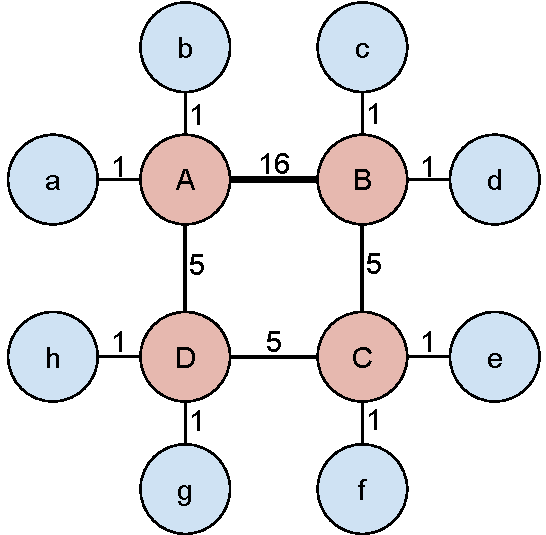
\includegraphics[width=0.8\linewidth]{images/testes_topo_uneven.pdf}
    \caption{Topologia simétrica com um \textit{link} custoso.}
    \label{fig:tested_topologies:small}
\end{subfigure}
\begin{subfigure}{.5\textwidth}
    \centering
    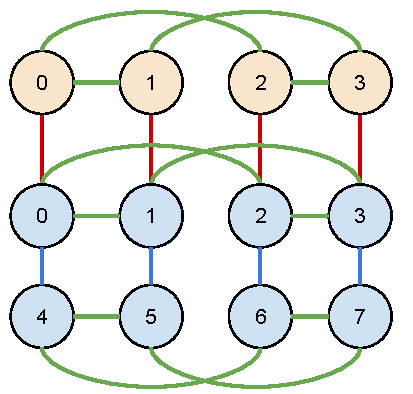
\includegraphics[width=0.8\linewidth]{images/testes_real_topo_no_links.pdf}
    \caption{Topologia assimétrica. \textit{Links} azuis, verdes e vermelhas têm custo 1, 2 e 8, respectivamente.}
    \label{fig:tested_topologies:real}
\end{subfigure}
\caption[Topologias utilizadas para teste.]{Topologias utilizadas para teste.}
\label{fig:tested_topologies}
\end{figure}

A Figura~\ref{fig:tested_topologies} apresenta duas topologias utilizadas para testar as funcionalidades da abstração.
Como a inicialização das topologias foi manual, não foram utilizadas topologias muito grandes.
A topologia (a) tem como objetivo verificar o funcionamento correto dos métodos de distância e \hops.
A topologia (b) apresenta um ambiente heterogêneo e um maior detalhamento da estrutura interna de cada máquina, permitindo observar a divisão adequada entre topologia de máquina e de rede feita pela abstração.
Para avaliar um funcionamento mais extenso na topologia de rede, a topologia (b) é utilizada novamente considerando cada PE como uma máquina individual.

As funcionalidades cobertas pelos testes são: (1) número de PEs na topologia; (2) número de máquinas na topologia; (3) PEs de uma máquina; (4) máquina de um determinado PE; (5) nó de um determinado PE; (6) outros PEs na máquina de um determinado PE; (7) PEs em uma determinada máquina; (8) outros PEs no mesmo nó de um determinado PE; (9) PEs em um determinado nó; (10) número de \links na camada de rede; (11) nome da topologia; (12) mudança de nome da topologia; (13) vizinhos na camada de rede; (14) proximidade entre dois PEs; (15) distância mínima entre dois PEs; (16) \textit{hops} entre dois PEs; (17) serialização de uma topologia; (18) leitura de uma topologia; (19) inicialização de uma topologia; e (20) persistência de informações entre execuções.

Em relação às estruturas utilizadas foram cobertas as seguintes funcionalidades: (1) criação de um CSC com um mecanismo de memoização; (2) inserção em um CSC; serialização de um CSC; (3) cálculo de distância mínima em um CSC; (4) utilização da memoização no cálculo de distâncias do CSC; (5) criação de uma matriz triangular superior sem diagonal; (6) inserção em uma matriz triangular superior sem diagonal; e (7) serialização de uma matriz triangular superior sem diagonal.

%Para garantir que não há escapamento de memória ou leituras invalidas, foi utilizada a ferramenta \textit{valgrind}.

\section{Balanceador de Carga}
\label{sec:my_lb}

% Porque usar um balanceador de carga
% porque usar este balanceador de carga
% O que faz esse balanceador
% o que foi modificado nesse balanceador

Para a demonstração do funcionamento da abstração da topologia de rede, foi modificado um balanceador de carga distribuído presente na plataforma \charm, de nome NeighborLB.
A modificação realizada só alterou de onde as informações de topologia foram retiradas, substituindo a implementação nativa pela Net Topo, sendo que o algoritmo do balanceador não foi alterado.
Este balanceador observa somente PEs vizinhos para a tomada de decisão de balanceamento, evitando contenção da rede e obtendo baixa latência nas mensagens.
Assim como outros balanceadores distribuídos, o NeighborLB  é escalável, pois independe do número de nós da rede. Porém, seu balanceamento é limitado pela quantidade de informação.

O descobrimento de vizinhos no balanceador NeighborLB é dado através de um balanceador base que existe dentro da plataforma \charm que utiliza seu mecanismo de inferência.
Este mecanismo foi substituído pela abstração criada para comprovar seu funcionamento.

A escolha do balanceador NeighborLB se deu pela sua simplicidade e por observar somente seus vizinhos, criando um cenário de comparação equivalente para a abstração Net Topo.
Os métodos de cálculo de \hops do \charm são mais velozes por considerarem topologias especificas (e as vezes imprecisas), o que causaria um cenário onde não se poderia avaliar o sobrecusto da abstração de maneira equivalente.
Nenhum dos balanceadores que utiliza as informações topológicas do \charm possui um cálculo de distância, por não possuir nenhuma informação de latência, inviabilizando a comparação neste nível.
% avaliam um unico core, de uma unica maquina, comparando diferentes topologias para ver como trabalha em escalas diferentes. Pode ter uso 

%mas eu vou tirar informação do charm pra por de novo? > facilidade no acesso, sem ter de realizar de novo


\section{Avaliação de Sobrecusto}
\label{sec:overhead}

% Porque avaliar o sobrecusto
% Como que foi feita essa avaliação

Para observar o sobrecusto da abstração, foi comparada a execução do balanceador NeighborLB, detalhado na Seção~\ref{sec:my_lb}, com o balanceador myNeighborLB, uma modificação do anterior que utiliza a Net Topo em vez do sistema topológico do \charm.
O objetivo da comparação é observar se há uma discrepância de desempenho no uso da abstração, verificar o uso funcional das abstração junto ao modulo de balanceamento de carga do \charm e observar possíveis ganhos e perdas de desempenho da abstração.

O \textit{benchmark} sintético \textit{LB Test} foi utilizado para realizar uma avaliação da execução dos balanceadores de carga.
Nele são criadas cargas uniformemente distribuídas entre uma valor de carga mínimo e máximo. 
O \textit{LB test} cria um perfil de comunicação entre estas cargas e invoca um balanceador de carga periodicamente, ambos escolhidos pelo usuário.
As configurações do \textit{LB test} são abordadas na Subseção~\ref{subsec:casos_exec}.
O ambiente de execução do \textit{benchmark }é determinado por um arquivo de grupos de execução, contendo as máquinas que serão utilizadas e seus IPs.
No caso deste trabalho, as máquinas Ciclope e Centauro foram utilizadas, detalhadas a seguir.

\subsection{Ambiente de Execução}
\label{subsec:ambiente}

% Onde é executado

A execução foi realizada em um conjunto de duas máquinas diferentes: (i) Ciclope e (ii) Centauro.
A primeira máquina utiliza 4 CPUs Intel Core i7-7700 @3.60GHZ com \textit{hypertreading} e possui 8GB@1200 MHz de memória. Possui 3 níveis de cache com tamanhos de 32 KB, 256 KB e 8 MB.
Sua versão de GCC é 5.5.0.
A segunda máquina possui 4 CPUs Intel Core i5-7400 @3.00GHz e 16GB@2400 MHz DIMM de memória. Possui 3 níveis de cache com tamanhos de 32 KB, 256 KB e 6 MB. GCC instalado na versão 5.4.0.
Ambas as máquinas utilizam Linux Mint na versão 18.2 e \charm 6.9.0.
A Figura~\ref{fig:run_topology} apresenta a topologia de cada máquina e do ambiente como um todo. 


\begin{figure}[h]
\begin{subfigure}{.6\textwidth}
    \centering
    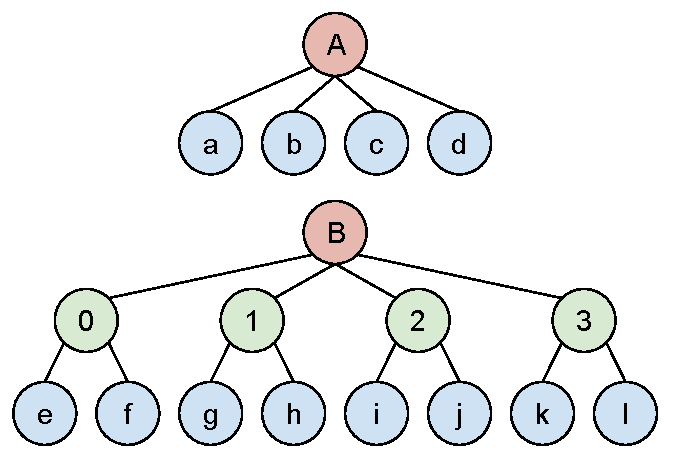
\includegraphics[width=0.8\linewidth]{images/init_real_topo.pdf}
    \caption{Em vermelho os agrupamento das máquinas Centauro (A) e Ciclope (B). Em verde os agrupamentos de \textit{cache}.}
    \label{fig:exec:machine_topos}
\end{subfigure}
\begin{subfigure}{.4\textwidth}
    \centering
    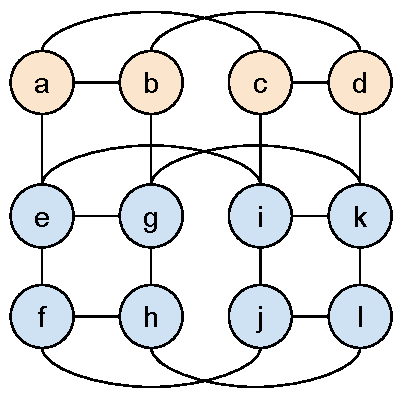
\includegraphics[width=0.8\linewidth]{images/execucao_topo.pdf}
    \caption{Topologia de rede do ambiente. Círculos azuis representam os PEs da máquina Ciclope e em laranjas os da máquina Centauro.}
    \label{fig:exec:full_topos}
\end{subfigure}
\caption[Topologia das máquinas Ciclope e Centauro.]{Topologia do ambiente de execução. Os agrupamentos de cada máquina  estão em (a) e a topologia de rede em (b).}
\label{fig:run_topology}
\end{figure}

\subsection{Casos de Execução}
\label{subsec:casos_exec}
% Quais testes vão ocorrer
% Como que os testes vão ocorrer
% Como foram realizados
% O que medem

Foram realizados três configurações do \textit{LB test} para realizar os experimentos capturados neste trabalho, com os seguintes nomes: (i) \textit{init}, (ii) \textit{LB test M} e (iii) \textit{LB test G}.
A Tabela~\ref{tab:execution_count} apresenta o nome de cada configuração e o número de execuções de cada uma delas.
A primeira configuração visa observar os tempos de inicialização da abstração de topologia Net Topo, do armazenamento dela, da inicialização da topologia nativa do \charm e da inicialização através de um arquivo XML. 
Portanto, não é preciso executar nenhum balanceamento de carga e o \textit{LB test} foi utilizado por conveniência.
As configurações (ii) e (iii) visam observar variação no desempenho do balanceador.
Em ambas foi utilizada uma execução de 150 iterações com o balanceador sendo invocado a cada 40 iterações, o intervalo de carga foi de 30 a 4120ms e o padrão de comunicação utilizado foi de anel.
A diferença entre as configurações (ii) e (iii) é o número de tarefas criadas.
Na configuração \textit{LB test M} foram criadas 3600 tarefas (300 tarefas por PE) enquanto na configuração \textit{LB test G} este número foi aumentado para 5400 (450 tarefas por PE).
A execução de dois níveis de carga diferentes visa observar alguma mudança devido ao Net Topo e relativa a carga, que não deveria ocorrer.

Por fim, as três configurações foram executadas no ambiente Ciclope + Centauro com a opção de execução ``\textit{++LBtestPESpeed}'' que permite que balanceadores coletem e utilizem a velocidade das CPUs de cada máquina para o balanceamento.

\setlength{\tabcolsep}{0.5em}
\begin{table}[!ht]
    \centering
    \begin{tabular}{l c}
        \toprule
        \textbf{Nome} &    \textbf{Número de execuções} \\ \midrule
        \textit{Init} & 120   \\ %\hline
        \textit{LB test M} & 20   \\ %\hline
        \textit{LB test G} & 15 \\ \bottomrule
    \end{tabular}
    \caption[Configurações de execução]{Nome das configurações e seu número de execuções.}
    \label{tab:execution_count}
\end{table}

\subsection{Resultados}
% O que vai ser visto
% porque dividir

Os resultados foram divididos em (i) inicialização (ii) e balanceamento de carga.
Na primeira parte (inicialização) é avaliada a configuração \textit{init}, observando os custos de inicialização de estruturas para a execução.
Na segunda parte (balanceamento de carga) é observado os sobrecustos da utilização da Net Topo utilizando as configurações \textit{LB test M} e \textit{LB test G} com os balanceadores NeighborLB (NLB) e myNeighborLB (myNLB).

\subsubsection{Inicialização}
% O que foi observado
% O que cada comparação gera

Na configuração de \textit{init} foram observadas quatro inicializações: (i) a Nativa do \charm, (ii) a do Net Topo, (iii) a integração destas duas e (iv) a inicialização Net Topo com um arquivo XML.
A inicialização (i) realiza uma série de mensagens IP entre as máquinas, encontrando e identificando cada PE de cada máquina as enquadrando para uma das topologia internas.
A (ii) coleta as informações da topologia do \charm, as organiza para a estrutura do Net Topo e as armazena, salvando tudo em um arquivo XML.
Como esta inicialização é dependente da nativa, a soma das duas também foi calculada como a inicialização (iii).
Por último, a importação XML (iv) captura as informações armazenadas por uma inicialização anterior do Net Topo.

% init padrao do charm: media 0.024s, desvio de 18,8%, 30 amostras
% mytopo start: media 0.0008888s, desvio de 38,2%, 30 amostras
% load topology: media: 0.000725, desvio de 8,8%, 35 amostras

\setlength{\tabcolsep}{0.5em}
\renewcommand{\arraystretch}{1.1}
\begin{table}[!ht]
    \centering
    \begin{tabular}{l c c}
        \toprule
        \textbf{Inicialização} & \textbf{Tempo médio de execução (ms)} & \textbf{Desvio Padrão (ms)} \\ \midrule
        Nativa do \charm & 24,46 & 5,22   \\ 
        Net Topo & 0,87 & 0,18   \\ 
        Nativa + Net Topo & 25,33 & 5,41   \\ 
        Importação XML & 0,72 & 0,06 \\ \bottomrule
    \end{tabular}
    \caption[Inicializações e seus desempenhos]{Inicializações testadas, seus tempos de execução e seu desvio padrão.}
    \label{tab:init_times}
\end{table}

A Tabela~\ref{tab:init_times} apresenta o tempo e desvio padrão de cada uma das inicializações observadas. 
Quando comparada com a nativa, a adição da inicialização da Net Topo gerou em média 3.5\% de sobrecusto.
É importante ressaltar que apesar da inicialização da Net Topo ter tido uma grande variância, quando somada a execução nativa não aumentou o desvio padrão.
Quando comparada a nativa, a importação XML reduz em média o tempo de inicialização em 97.1\%, agilizando o processo de inicialização do sistema.
Conforme o número de PEs do sistema aumenta, é esperado que este ganho entre a importação e a inicialização cresça ainda mais, pois a implementação nativa realiza uma multitude de mensagens IPs para encontrar e definir a topologia.
Por outro lado, o custo de inicialização da Net Topo deve crescer junto com o número de PEs. Não se sabe se o sobrecusto dela irá se manter, aumentar ou reduzir quando adicionada a nativa, mas se o desempenho da importação se mantiver, é provável que o sobrecusto de inicialização do Net Topo se pague na segunda execução.

\subsubsection{Balanceamento de Carga}

Nas configurações \textit{LB test M} e \textit{LB test G} foram capturadas duas informações para comparação: (i) o tempo de balanceamento e (ii) o tempo de execução da aplicação.
A primeira informação permite observar modificações na velocidade do balanceador, a análise deste busca observar o sobrecusto da abstração.
A segunda avalia mudanças no balanceamento da aplicação, que não deveria ser afetado, pois não há mudanças no comportamento do balanceador.

Na Tabela~\ref{tab:lb_times} é observado o tempo e o desvio padrão de balanceamento de NLB e de myNLB nas configurações de teste \textit{LB test M} e \textit{LB test G}.
Ambos as configurações apresentaram uma melhora na abordagem com Net Topo, com uma redução de tempo de 0.18 ms e 0.19 ms, respectivamente. Como esta pequena melhoria não escalou, significa que não é dependente da quantidade de carga, a diferença entre as configurações.
Essa melhoria indica que a abstração criada oferece um acesso a vizinhos ligeiramente mais rápida que a nativa do \charm, pois ambas as execuções e realizam o mesmo número de invocações para encontrar vizinhos.

% lb time: média 0.01960, 14,5% de desvio, 60 amostras
% my_lb time: média 0.01942, 14,3% de desvio, 60 amostras
% big lb time: 0.02912, 14,5% de desvio, 45 amostras
% big my lb: 0.02893, 13,2% de desvio, 45 amostras
\setlength{\tabcolsep}{1.0em}
\renewcommand{\arraystretch}{1.2}
\begin{table}[!ht]
    \centering
    \begin{tabu}{ l c c c c}
        \toprule
        \multirow{2}{*}{Configuração} & \multicolumn{2}{c}{\textit{LB test M}} & \multicolumn{2}{c}{\textit{LB test G}} \\
         & \textit{NLB} & \textit{myNLB} & \textit{NLB} & \textit{myNLB}\\ \midrule
        Tempo médio de balanceamento (ms) & 19,60 & 19,42 & 29,12 & 28,93   \\  
        Desvio Padrão (ms) & 2,85 & 2,78 & 4,22 & 3,83 \\ \bottomrule
    \end{tabu}
    \caption[Tempo de balanceamento de carga]{Tempo médio de balanceamento de carga e desvio padrão dos balanceadores NeighborLB e myNeighborLB nos casos de execução \textit{LB test M} e \textit{LB test G}.}
    \label{tab:lb_times}
\end{table}


% neighbor time: media: 66.217s, 6,9% de desvio, 20 amostras
% my neighbor_time: média 65.188s, 9,5% de desvio, 20 amostras
% neighbor time big: media: 92,768, 7,85% de desvio, 15 amostras
% my neighbor time big: média: 91,220, 10.1% de desvio, 15 amostras
Os resultados de tempo dos balanceadores de carga são observados no gráfico da Figura~\ref{fig:exec_times}. Surpreendentemente, a versão modificada obteve em média uma pequena melhoria no tempo total de execução (de aproximadamente 1,5\%). 
As melhorias no tempo de balanceamento não geram tanto impacto (totalizam menos de 1ms no total) e o tempo de inicialização não é considerado no tempo da aplicação.
O motivo atribuído a melhoria é a natureza variante do \textit{benchmark} acoplado com número baixo de execuções e um desvio padrão próximo a 10\% nas execuções.
O que se conclui aqui é que não houve mudanças significativas no comportamento do balanceador.
\begin{figure}[h]
    \centering
    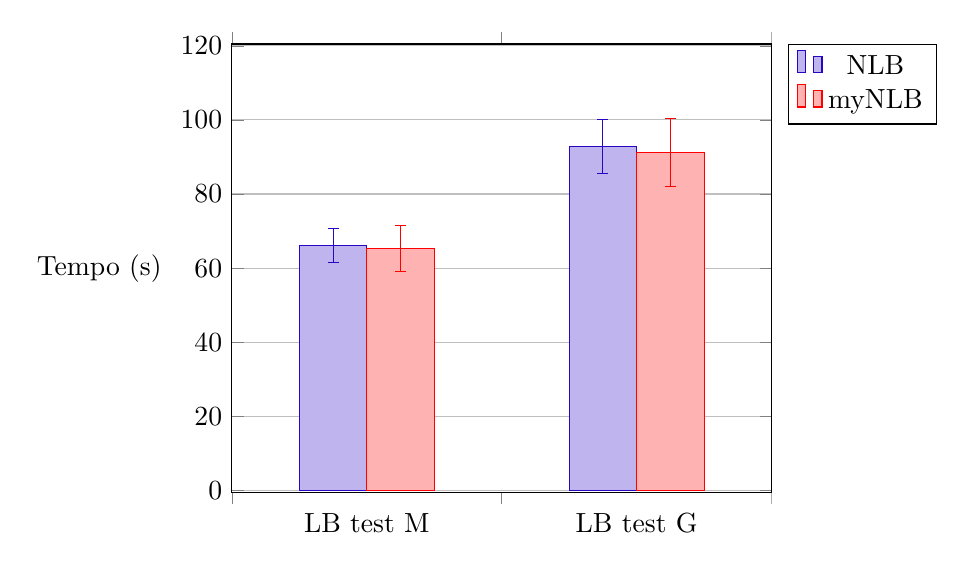
\begin{tikzpicture}
    \begin{axis}[
    legend pos=outer north east,
    enlargelimits={abs=0.5},
    ylabel style={rotate=-90},
    ylabel={Tempo (s)},
    ybar=0pt,
    ymajorgrids=true,
    bar width=0.25,
    ymin=0, ymax=120,
    xtick={0.5, 1.5, 2.5, 3.5 , 4.5},
    xticklabels={LB test M, LB test G, 5},
    x tick label as interval,
    ]
    
    \addplot+[error bars/.cd,
    y dir=both,y explicit]
    coordinates {
        (1, 66.21) +- (0.0, 4.59)
        (2, 92.76) +- (0.0, 7.29)};
    \addplot+[error bars/.cd,
    y dir=both,y explicit]
    coordinates {
        (1, 65.18) +- (0.0, 6.21)
        (2, 91.22) +- (0.0, 9.21)};
    
    \legend{NLB, myNLB}
    \end{axis}
    \end{tikzpicture}
    \caption[Comparação de tempos de balanceamento entre NeighborLB e myNeighborLB.] {Comparação de tempos de balanceamento entre NeighborLB e myNeighborLB. Os intervalos em cada barra representam o desvio padrão.}
    \label{fig:exec_times}
\end{figure}

As execuções realizadas com o \textit{benchmark LB test}, o balanceador NeighborLB e sua modificação para utilizar a Net Topo permitiram observar: (i) um sobrecusto de 3,5\% na inicialização do \charm, compensado largamente pelo ganho significativo na inicialização com XML; (ii) um sobrecusto abaixo do esperado no balanceamento, inclusive com menos custo que o do próprio \charm; e (iii) não houve um impacto negativo na qualidade do balanceamento, já que o algoritmo não foi modificado.
Estes resultados permitem afirmar o funcionamento desejado pela abstração.
Por outro lado, os experimentos realizados são bem limitados, pois observam uma escala reduzida de apenas duas máquinas e 12 PEs, o que inviabiliza assunções seguras em relação ao sobrecusto para outras escalas de aplicação.
Outra limitação dos experimentos é a avaliação de somente a função de vizinhança da abstração, não podendo, por exemplo, indicar o sobrecusto de se considerar uma topologia genérica em um cálculo de \textit{hops}.


% observar os ganhos com importação
% comentar as estruturas
%falar o escopo de avaliação limitada

\section{Avaliação de Desempenho}
\label{sec:bench}

Para observar o funcionamento da abstração em escalas diferentes, foi criado um gerador de topologias \fatt, \textit{mesh2D} e \textit{mesh3D} e observado os tempos de execução de 4 topologias geradas. 
Estes casos são apresentados na Seção~\ref{sec:bench:cases}.
A Tabela~\ref{tab:sizes_bench} apresenta as funcionalidades avaliadas e o número de execuções de cada uma. 
A função de inicialização é representada por \textit{init}, as de arquivamento e importação XML por \textit{save} e \textit{load}, respectivamente, e a de preenchimento do mecanismo de memoização por \textit{fill}.
Os cálculos de proximidade são detalhados logo antes de seus respectivos experimentos.

\setlength{\tabcolsep}{0.5em}
\begin{table}[!ht]
    \centering
    \begin{tabular}{l c}
        \toprule
        \textbf{Métodos} &    \textbf{Número de execuções} \\ \midrule
        \textit{init}, \textit{save} e \textit{fill} & $25$   \\ %\hline
        \textit{load} & $100$   \\ %\hline
        cálculos de proximidade & $200$ \\ \bottomrule
    \end{tabular}
    \caption[Número de execuções de cada função.]{Número de execuções de cada função testada. Um dos cálculos de proximidade foi executado 100 vezes em vez de 200.}
    \label{tab:sizes_bench}
\end{table}

A execução dos testes foi realizada na máquina Centauro, apresentada na Seção~\ref{subsec:ambiente}, utilizando um único núcleo e medindo o tempo através da biblioteca \textit{crono} de \textit{C++}.
Não foi utilizado um ambiente maior ou paralelo, pois o objetivo da execução era observar a variação de desempenho da estrutura em escalas diferentes.


% a velocidade não é questionada.
% valores de hop 1 e dist 1 não foram apresentados pois aprezentam valores de desvio padrão superior a 100%.

% definir cada coisa sendo testada, como vizinhança II
\subsection{Casos de Execução}
\label{sec:bench:cases}

Foram criados 4 casos de representações de topologias para a execução dos testes: uma \fatt com 7 níveis, nomeada de \textit{tree M}; uma \fatt de 10 níveis, representada como \textit{tree G}; uma \textit{mesh2D} de tamanho 16x16,  representada por \textit{mesh2D}; e uma \textit{mesh3D} simétrica de dimensão 8, nomeada \textit{mesh3D}.
Todas as topologias tiveram uma versão da abstração com memoização e outra sem. 
O número de máquinas e ligações de cada um dos casos de teste estão apresentados na Tabela~\ref{tab:sizes_topos}.
A coluna tamanho do arquivo XML e XML- representa o espaço em disco do arquivo XML gerado pela Net Topo com e sem memoização, respectivamente.
É possível observar que este tamanho não escala bem devido ao dispositivo de memoização, por ocupar espaço com complexidade $O(m^2)$ onde $m$ é o número de maquinas.

\setlength{\tabcolsep}{0.5em}
\begin{table}[!ht]
    \centering
    \begin{tabular}{l c c c c}
        \toprule
        \textbf{Caso} &    \textbf{Número de máquinas}  & \textbf{Número de ligações}  & \textbf{XML/M} & \textbf{XML} \\ \midrule
        \textit{tree M} & 127 & 126   & $0,32$  & $0,05$ \\ %\hline
        \textit{mesh2D} & 256 & 538   & $1,28$  & $0,12$  \\ %\hline
        \textit{mesh3D} & 512 & 1.344  & $5,06$  & $0,31$  \\ %\hline
        \textit{tree G} & 1.023 & 1.022 & $20,06$ & $0,42$  \\ \bottomrule
    \end{tabular}
    \caption[Tamanho das topologias]{Tamanho das abstrações criadas em número de máquinas, em número de ligações e em ocupação do arquivo XML em MB com e sem memoização, representado por XML/M e XML, respectivamente.}
    \label{tab:sizes_topos}
\end{table}

% execuções
% inicialização, save, fill: 25
% load, dist_2: 100
% hops, prox: 200
\subsection{Resultados}

Os resultados dos experimentos foram divididos em duas partes: (i) inicialização e serialização e (ii) cálculos de proximidade.
A primeira parte contempla os tempos de inicialização, arquivamento e importação XML de cada um dos casos.
A segunda compara os tempos de cálculo de proximidade, \hops e distância de cada um dos casos e do preenchimento do mecanismo de memoização nos casos que possuem memoização.
Para reduzir o desvio padrão e apresentar um resultado mais coerente, foram retirados da amostra casos discrepantes que ocorreram com baixa frequência (1\% ou menos) pois alteravam a média e o desvio padrão de maneira significante por serem valores de duas ordens de grandeza a mais.

\subsubsection{Inicialização e Serialização}

A Figura~\ref{fig:init_bench} apresenta o crescimento do tempo médio de inicialização, arquivamento e importação XML de cada um dos casos com o crescimento de número de máquinas.
As topologias \textit{tree M}, \textit{mesh2D}, \textit{mesh3D} e \textit{tree G} são representadas por $2^7$, $2^8$, $2^9$ e $2^{10}$ máquinas, respectivamente.
É possível observar que, quando sem memoização, os tempos de arquivar e importar crescem linearmente ou sublinearmente com a quantidade de máquinas.
Por outro lado é fácil observar que o mecanismo de memoização em forma de matriz não escala bem com o tamanho da topologia devido a sua natureza quadrática.
Isso se deve pelo fator da matriz de memoização representar metade de todas a ligações possíveis, que são mais de 524 mil no caso \textit{tree G}.

\begin{figure} [h]
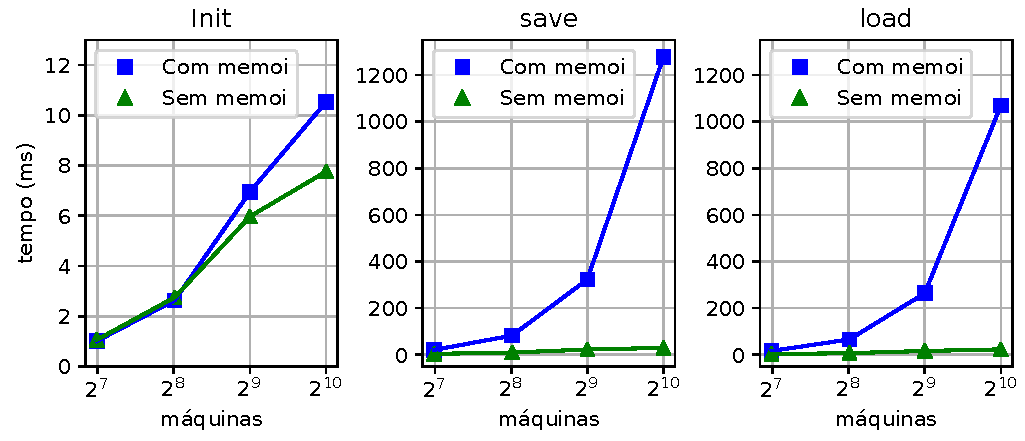
\includegraphics[width=1.02\textwidth]{images/init_save_load.pdf}
\centering
\caption[Tempos de inicialização, arquivamento e importação XML.] {Crescimento dos tempo médio de inicialização (init), arquivamento (save) e importação XML (load) de cada um dos casos de teste. Os quadrados em azul são os casos com memoização e os triângulos em verde os casos sem memoização. }
\label{fig:init_bench}
\end{figure}

% \setlength{\tabcolsep}{0.5em}
% \begin{table}[!ht]
%     \centering
%     \begin{tabular}{| l | c | c | c |}
%         \toprule
%         \textbf{Caso} &    \textbf{\textit{init}} (ms) & \textbf{\textit{save}} (ms) & \textbf{\textit{load}} (ms)\\ \hline

%         \textit{tree M-}    & $1,06$ $(0,14)$   & $2,84$ $(0,24)$    & $3,89$ $(0,13)$  \\ \hline
%         \textit{tree M}     & $1,01$ $(0,01)$   & $16,46$ $(1,15)$     & $20,94$ $(0,06)$  \\ \hline
%         \textit{mesh2D-}    & $2,75$ $(0,18)$   & $6,98$ $(0,25)$     & $9,62$ $(0,19)$   \\ \hline
%         \textit{mesh2D}     & $2,63$ $(0,01)$   & $65,92$ $(3,64)$      & $82,38$ $(0,28)$   \\ \hline
%         \textit{mesh3D-}    & $5,97$ $(0,05)$   & $16,35$ $(0,16)$    & $22,47 $ $(1,01)$  \\ \hline
%         \textit{mesh3D}     & $6,95$ $(3,05)$  & $263,78$ $(10,31)$    & $322,76$ $(1,38)$   \\ \hline
%         \textit{tree G-}   & $7,75$ $(0,16)$   & $23,14$ $(0,83)$      & $29,82$ $(0,15)$   \\ \hline
%         \textit{tree G}    & $10,53$ $(5,56)$ & $1.068,07$ $(38,45)$   & $1.276,68$ $(8,04)$   \\ 
%         \bottomrule
%     \end{tabular}
%     \caption[Tempos de inicialização, arquivamento e importação XML.]{Tempos médios de inicialização, arquivamento e importação XML de cada um dos casos de teste. Desvio padrão entre parenteses.}
%     \label{tab:init_bench}
% \end{table}

\subsubsection{Cálculos de Proximidade}

A função de proximidade é um cálculo que avalia a proximidade entre dois PEs, observando se estão na mesma máquina ou não.
O tempo médio de um cálculo de proximidade foi entre 0,20 e 0,21 microssegundos em todos os casos de execução. 
O desvio padrão foi entre 0,04  e 0,06 microssegundos em todos os casos.
Foi observado que o cálculo de proximidade independe do tamanho da topologia e de ter ou não memoização, como era esperado.

O cálculo de distância avalia a latência entre duas máquinas da topologia.
Para avaliar a latência deste cálculo, foi agrupado o tempo de todos os cálculos de distância entre uma máquina e todas as máquinas a até dois \hops de distância dela. 
Este conjunto de distâncias calculadas foi denominado como ``distância II''.

O cálculo da distância II utiliza o mecanismo de memoização, e foram avaliados três cenários relativos a memoização: (i) inicialmente completa, (ii) inicialmente vazia e (iii) sem nenhum tipo de memoização.
A primeira contêm todas as informações de distância calculadas previamente.
A segunda inicia cada cálculo com a memoização inicialmente vazia, expandindo durante a execução de uma distância II.
O terceiro caso não utiliza nenhuma memoização e é utilizada para comparação.

A Tabela~\ref{tab:dist_comparison} apresenta os tempos médios de execução do preenchimento da matriz de memoização e dos três cenários de distância II.
A primeira coluna apresenta o tempo de preenchimento, que é o tempo o mecanismo de memoização através de cálculos de distância entre todos os nós.
A primeira linha de cada caso de execução indica a média dos tempos e a segunda linha o desvio padrão.

\setlength{\tabcolsep}{0.5em}
\begin{table}[!ht]
    \centering
    \begin{tabular}{l c c c c c}
        \toprule
        \textbf{Caso} & &   \textbf{Preenchimento} (ms)  & \textbf{Completa} ($\mu$s) & \textbf{Vazia} ($\mu$s) & \textbf{Sem memoização} ($\mu$s)\\ \midrule
        \multirow{2}{*}{\textit{tree M}}  & $\overline{x}$   & $75,70$   & $1,30$     & $11,32$    & $50,56$  \\
        & $\sigma$ & 0,98 & 0,04 & 4,68 & 13,15 \\ \hline
        \multirow{2}{*}{\textit{mesh2D}}  & $\overline{x}$   & $863,91$  & $2,69$     & $75,72$    & $210,42$   \\
        & $\sigma$ & 5,70 & 0,04 & 24,04 & 41,77 \\ \hline
        \multirow{2}{*}{\textit{mesh3D}}  & $\overline{x}$   & $4.880,94$   & $4,96$      & $214,90$   & $873,95$   \\
        & $\sigma$ & 19,03 & 0,35 & 21,12 & 77,39 \\ \hline
        \multirow{2}{*}{\textit{tree G}}  & $\overline{x}$  & $6.215,44$ & $1,40$    & $16,63$    & $39,49$   \\
        & $\sigma$ & 24,24 & 0,06 & 5,74 & 9,63 \\ \bottomrule
    \end{tabular}
    \caption[Tempos de cálculo de distância da vizinhança II.]{O tempo médio ($\overline{x}$) e o desvio padrão ($\sigma$) de preenchimento completo da matriz de memoização (primeira coluna), e tempo do cálculo de distância II de uma máquina com memoização completa (coluna II), inicialmente vazia (coluna III) ou inexistente (última coluna).}
    \label{tab:dist_comparison}
\end{table}

Todos os cálculos de distância têm um desvio padrão aumentado devido a variação do grau de cada máquina, sendo de 1 a 3 em uma \fatt, 2 a 4 numa \textit{mesh2D} e 3 a 6 em uma \textit{mesh3D}.
O desvio padrão maior no caso de memoização inicialmente vazia se deve ao fator dos cálculos oscilarem entre encontrar um valor armazenado e encontrar um valor novo.

Como o número de distâncias possíveis cresce quadraticamente com o número de máquinas, o tempo de preenchimento também cresce quadraticamente. Este crescimento é observável na Tabela~\ref{tab:dist_comparison}. 
Para que este tempo de preenchimento acelere a execução, é necessário que seu tempo seja pago por um número grande de cálculos de distância. 
No caso \textit{tree M}, por exemplo, são necessárias 6180 execuções, enquanto para \textit{tree G} são necessárias 125845 execuções.


Quando comparado o tempo de preenchimento da \textit{mesh3D} com da \textit{tree G}, este não cresceu tanto quando comparado com o crescimento entre \textit{mesh2D} e \textit{mesh3D}, por realizar um cálculo de distância com um grau médio menor.
Portanto o tempo de preenchimento da memoização cresce tanto com o número de máquinas na topologia quanto com o tempo de um cálculo de distância.
Com isso, a quantidade de execuções de distância para que o preenchimento valha a pela varia para cada topologia.

É possível observar um aumento no tempo conforme o grau da topologia aumenta, assim como uma melhoria entre a completa para a inicialmente vazia e outra melhoria entre a inicialmente vazia e a sem memoização.
A  melhoria no caso da inicialmente vazia se deve ao algoritmo de distância armazenar a distância de todos os visitados, conseguindo encontrar a distância de uma parte da vizinhança nas primeiras execuções e utilizá-la nas seguintes.

Na Tabela~\ref{tab:avg_dist_comparison} são apresentados os tempos médios de cada cálculo de distância individualmente feito na distância II, em vez de um agrupamento destes.
O desvio padrão se encontra altíssimo devido a vários fatores, como a variância do grau na topologia, a oscilação entre com e sem memoização e a imprecisão de relógio devido a magnitude sendo avaliada.
Devido a esta alta imprecisão os valores são estatisticamente equivalentes e por isso foi avaliado o tempo de vizinhanças, que não tinha tanta variância.
Ainda assim, é possível constatar um pequeno crescimento no cálculo de cada distância com o crescimento do grau.

\setlength{\tabcolsep}{0.5em}
\begin{table}[!ht]
    \centering
    \begin{tabular}{l c c c c}
        \toprule
        \textbf{Caso} & &   \textbf{Completa} & \textbf{Vazia} & \textbf{Sem memoização}\\ \midrule
        \multirow{2}{*}{\textit{tree M}}  & $\overline{x}$   & $0,24$      & $2,05$    & $9,16$  \\ 
        & $\sigma$ & 0,03 & 4,78 & $13,15$ \\ \hline
        \multirow{2}{*}{\textit{mesh2D}}  & $\overline{x}$  & $0,25$       & $6,94$    & $19,28$   \\ 
        & $\sigma$ & 0,04 & 14,05 & $21,74$\\ \hline
        \multirow{2}{*}{\textit{mesh3D}}  & $\overline{x}$   & $0,26$     & $11,62$   & $45,82$    \\ 
        & $\sigma$ & 0,35  & 23,11 & 27,66 \\ \hline
        \multirow{2}{*}{\textit{tree G}}  & $\overline{x}$   & $0,27$      & $3,2$    & $7,71$   \\
        & $\sigma$ & 0,06 & 5,7 & 5,6 \\
        \bottomrule
    \end{tabular}
    \caption[Tempo médio de um cálculo de distância.]{O tempo médio ($\overline{x}$) e desvio padrão ($\sigma$) de um cálculo de distância com memoização completa, inicialmente vazia ou inexistente.}
    \label{tab:avg_dist_comparison}
\end{table}

% hops varia com tamanho do grau médio, tree_7 e tree_10 tiveram valores menores e similares, enquanto mesh2D e 3D tiveram um aumento

O cálculo de \hops é outra métrica para avaliar proximidade entre duas máquinas, observando o número mínimo de \links entre uma máquina e outra.
Assim como o cálculo de distância, foi realizado um cálculo de \hops entre uma máquina e todas as máquinas a até dois \hops de distância, agrupando seus tempos num valor denominado de \hops II.
Esse agrupamento foi utilizado para estabilizar os valores, sendo que é possível encontrar a segunda vizinhança com \hops de maneira muito mais ágil.

Os tempos de \hops II são apresentados na Tabela~\ref{tab:dist_hop}, comparados com o tempo de distância II.
Assim como o cálculo de distância, os cálculo de \hops demonstrou um aumento no tempo de execução devido ao aumento do grau médio.
Não era esperado que os tempo de execução variasse com o número de máquinas, como ocorreu com a \textit{tree G}.

\setlength{\tabcolsep}{0.5em}
\begin{table}[!ht]
    \centering
    \begin{tabular}{l c c c c}
        \toprule
        \textbf{Caso}   &    & \textbf{Hops} ($\mu$s) &    \textbf{Distância} ($\mu$s) & \textbf{Sem memoização} ($\mu$s)\\ \midrule
        \multirow{2}{*}{\textit{tree M}} & $\overline{x}$    & $23,50$   & $11,32$  & $50,56$   \\ 
        & $\sigma$ & 6,36 & 4,68 & 13,15\\ \hline
        \multirow{2}{*}{\textit{mesh2D}} & $\overline{x}$    & $85,11$   & $75,72$ & $210,42$  \\
        & $\sigma$ & 13,39 & 24,04 & 41,77 \\ \hline
        \multirow{2}{*}{\textit{mesh3D}} & $\overline{x}$    & $534,50$  & $214,90$ & $873,95$  \\
        & $\sigma$ & 7,53 & 21,12 & 77,39 \\ \hline
        \multirow{2}{*}{\textit{tree G}} & $\overline{x}$     & $39,23$    & $16,63$ & $39,49$   \\
        & $\sigma$ & 2,46 & 5,74 & 9,63 \\ \bottomrule
    \end{tabular}
    \caption[Comparação entre hop e distância para vizinhança II.]{Comparação do tempo médio ($\overline{x}$) e desvio padrão ($\sigma$) de \hops II e distância II.}
    \label{tab:dist_hop}
\end{table}

Era esperado que o cálculo de \hops fosse mais rápido que o cálculo de distância em todos os casos mas, como não foi utilizado memoização para \hops, alguns casos de distância foram mais rápidos quando o grau médio foi elevado.
Isso se dá pelo armazenamento da distância de múltiplos vizinhos em um único cálculo de distância.
É possível observar que houve um acréscimo no tempo do cálculo de \hops, provavelmente devido a uma redução de localidade da cache.

Por fim, a Tabela~\ref{tab:memoi_worth} apresenta a aceleração do mecanismo de memoização na serialização e na distância II com memoização completa ou inicialmente vazia.
É importante que, mesmo com uma aceleração grande na distância, o tempo de preenchimento da memoização pode fazer com que não valha a pena.
No caso da \textit{tree G}, por exemplo, seria necessário em torno 164 mil execuções de distância II para que a redução no tempo comece a ser um benefício.

\setlength{\tabcolsep}{0.5em}
\begin{table}[!ht]
    \centering
    \begin{tabular}{l c c c c}
        \toprule
        \textbf{Caso}       & \textbf{\textit{save}} &    \textbf{\textit{load}} & \textbf{Vazia} & \textbf{Completa}\\ \midrule
        \textit{tree M}     & $0,172$   & $0,185$ & $4,46$ & $38,89 $ \\
        \textit{mesh2D}     & $0,105$   & $0,116$ & $2,77$ & $78,22$ \\
        \textit{mesh3D}     & $0,061$   & $0,069$ & $4,06$ & $176,00$  \\ 
        \textit{tree G}     & $0,021$   & $0,023$ & $2,37$ & $28,21$ \\ \bottomrule
    \end{tabular}
    \caption[Aceleração da memoização.]{Aceleração geradas pela memoização como matriz superior. As colunas \textit{save} e \textit{load} apresentam os atrasos no tempo médio de arquivamento e importação, respectivamente. As colunas \textit{Vazia} e \textit{Completa} apresentam a aceleração no tempo médio de distância II com memoização inicialmente vazia e completa, respectivamente. }
    \label{tab:memoi_worth}
\end{table}

Estes experimentos avaliaram o funcionamento da Net Topo em escalas diferentes e o impacto da memoização implementada.
Foi possível determinar que a memoização em forma de matriz não é escalável, causa um detrimento considerável no tempo para o arquivamento e importação e para que seu preenchimento valha a pena, seria necessário um número muito alto de execuções.
Apesar disso, ela gera uma aceleração considerável na execução do cálculo de distâncias de uma vizinhança, mesmo quando inicialmente vazia, mas este benefício depende do grau médio da topologia.
Em relação a escalabilidade da abstração, os tempos de inicialização, serialização, e proximidade escalaram de maneira adequada, mas os cálculos de distância e \hops cresceram ligeiramente com o número de máquinas, provavelmente devido a ocupação de memória.

\chapter{Conclusão}
\label{cap:conclusao}

Uma distribuição de carga ciente de topologia pode melhorar o desempenho de uma aplicação por considerar latências de comunicação e efeitos de contenção.
A obtenção de informações de topologia se dá através da coleta de informações dos sistemas em execução e troca de mensagens.
As ferramentas para obtenção destas informações têm limitações e inadequações para o contexto de escalonamento e balanceamento de carga, dificultando seu uso.

Neste trabalho foi desenvolvida a Net Topo, uma abstração de topologia que visa recolher e dispor informações da topologia de rede para uso em escalonamento e balanceamento de aplicações paralelas e distribuídas.
Dentre diversas opções de estruturas de dados e representação de topologia, foi utilizado um CSC, uma matriz de distâncias opcional e uma lista de árvores.
A abstração criada apresenta diversas informações de topologia e fornece funções de proximidade e distâncias, visando auxiliar o processo de distribuição de carga.
A Net Topo também possui diversos mecanismos para sua inicialização, incluindo implementações manuais e importação de um aquivo de topologia em XML.

Foi criado um adaptador para receber informações de inicialização e fazer uma ponte entre a abstração e o \textit{runtime} do \charm, permitindo utilizar a Net Topo junto ao módulo de balanceamento de carga presente na plataforma.
Para comprovar a integração e avaliar o sobrecusto da abstração, foi comparado um balanceador de carga com sua versão modificado para utilizar a Net Topo.
Apesar das execuções serem realizadas em baixa escala e em um ambiente pequeno, elas permitiram observar um sobrecusto de inicialização altamente compensado pelo arquivamento da topologia e pouca ou nenhuma mudança negativa nos tempos de execução do balanceador.
Foram realizados testes unitários para comprovar o uso de funcionalidades que não foram abrangidas no balanceador, de maneira que possam ser utilizadas independente da forma de inicialização da estrutura.

Por fim, foi implementado um gerador de topologias, avaliado o impacto da memoização e observado a escalabilidade da abstração.
O dispositivo de memoização através de uma matriz completa não se mostrou escalável, gerando sobrecustos muito altos conforme o tamanho da topologia cresce.
A função de proximidade se apresentou como constante e o restante das funções testadas demonstraram crescimento linear ou sublinear com o aumento no número de máquinas.

% que problema esse trabalho trata
% que solução foi apresentada
% apresentar os resultados 
% passar pelos objetivos 

\section{Trabalhos Futuros}
\label{sec:futuro}

A execução deste trabalho criou uma série de oportunidades de trabalhos futuros. Segue uma lista de extensões, melhorias e avaliações cogitadas:
\begin{itemize}
    \item Realizar uma distribuição das estruturas de topologia de modo que não seja puramente replicada em cada nó e reduza o espaço utilizado em cada máquina, mas ainda mantenha a possibilidade de uma travessia de grafo para cálculo de \hops ou latência.
    \item Modificar as estruturas da abstração para serem dinâmicas, possibilitando modificações e atualizações em uma topologia prévia, sem ter de reinicializá-la.
    \item Implementar uma inicialização utilizando informações do \hwloc para a topologia de máquina e o \charm para a topologia de rede, retirando as imprecisões relacionadas a máquinas do \charm enquanto se mantém a automatização do processo.
    \item Ampliar o gerador de topologias para a abstração, oferecendo casos de teste para uma gama maior de topologias.
    \item Executar testes de sobrecusto com balanceadores em escalas maiores, avaliando o sobrecusto de outras funcionalidades da Net Topo e como essa se comporta em outros ambientes.
    \item Buscar uma inicialização que contenha informações de latência entre pontos da rede, possivelmente utilizando \netloc.
    \item Aplicar um mecanismo de normalização para relativizar as distâncias na topologia, as deixando mais representativas para mecanismos de escalonamento e balanceamento.
    \item Produzir um mecanismo de agrupamento de regiões da rede, similar ao que foi feito para agrupamento de nós e máquinas, permitindo uma redução nos cálculos de distância e outro nível de proximidade, útil para redes no estilo \Dgfly que possuem partes da rede com latências distintas.
    \item Investigar alternativas ao uso de uma memoização como matriz e avaliar seus benefícios. Como por exemplo um mecanismo de cache um ou um uso de caminhos pré calculados.
\end{itemize}
% distribuir estrutura de maneira não replicada
% Dinamico
% Inicializar com Hwloc + charm para melhores informações
% Opção de retirar memoização
% Geradores de topologia para ampliar os casos de teste e uso
% agrupamento de rede

% investigar uso de uma memoização parcial em vez de completa




% ---


% 
\def\coordenador{Renato Cislaghi}
\def\orientador{Vinicius Marino Calvo Torres de Freitas}
\def\coorientador{Márcio Bastos Castro}
\def\autor{Thales Alexandre Zirbel Hubner}


\chapter{Planejamento}

Este capítulo contém o planejamento do projeto onde cada parte do plano de gerenciamento se encontra em seções diferentes. A Seção \ref{sec:cronograma} apresenta as atividades planejadas e seu cronograma a ser seguido ao longo da realização deste trabalho. A Seção \ref{sec:rh} apresenta os recursos humanos envolvidos. A Seção \ref{sec:custos} indica os custos estimados para a execução do projeto. A Seção \ref{sec:comunicacao} dispõe o gerenciamento da comunicação entre as partes envolvidas. A Seção \ref{sec:riscos} apresenta os riscos identificados e suas respectivas estratégias.

% ---
\section{Cronograma}
%\label{sec:cronograma}

As atividades previstas no projeto estão descritas abaixo:

\begin{itemize}
	\item \textbf{A1: Estudo da fundamentação teórica.} Nesta parte inicial será realizada a revisão de artigos e materiais relacionados a computação paralela, topologia de rede e balanceamento de carga.
	\item \textbf{A2: Familiarização com a plataforma charm++.} Processo de familiarização com a plataforma para programação paralela a ser utilizada.
	\item \textbf{A3: Revisão do estado da arte e prática.} Nesta etapa será tratada a revisão do estado da arte envolvido no contexto do trabalho, a fim de  fortalecer a base do conhecimento necessária para a realização do mesmo.
	\item \textbf{A4: Elaboração da proposta.} Nesta etapa será apresentada a proposta de solução do problema em questão, bem como suas estratégias de implementação.
	\item \textbf{A5: Escrita do relatório do TCC I.} Nesta etapa será realizada a escrita do relatório do TCC I. A entrega deste documento está prevista para a quarta semana do mês de novembro.
	\item \textbf{A6: Implementação da abstração da topologia de rede.} Nesta parcela será realizada a implementação da abstração proposta assim como a verificação do funcionamento desta.
	\item \textbf{A7: Teste da abstração da topologia de rede.} Nesta parcela será realizada a verificação do funcionamento da abstração.
	\item \textbf{A8: Desenvolvimento de um balanceador de carga.} Nesta etapa será efetuada o desenvolvimento de um balanceador de carga que utilize a abstração de rede criada.
	\item \textbf{A9: Testes e comparações de desempenho.} Nesta etapa será efetuado testes de desempenho do balanceador de carga a a comparação deste com outros balanceadores existentes.
	\item \textbf{A10: Escrita do rascunho do TCC II.} A escrita do rascunho do TCC II será realizada neste período. A entrega deste documento está prevista para a segunda semana do mês de maio.
	\item \textbf{A11: Preparação da defesa pública.} Nesta etapa será realizada a preparação da apresentação oral e visual do conteúdo deste trabalho para a defesa pública.
	\item \textbf{A12: Defesa pública.} Nesta etapa será realizada a defesa do projeto desenvolvido. Pretende-se realizar a defesa pública do trabalho na primeira semana do mês de junho.
	\item \textbf{A13: Correções e entrega da versão final do TCC.} Nesta etapa serão realizadas as correções e os ajustes da monografia e a entrega final do documento. A entrega da versão final está prevista para a quarta semana do mês de junho.
\end{itemize}

A Figura~\ref{fig:cronograma} apresenta o cronograma previsto para a realização das atividades descritas anteriormente. As atividades estão distribuídas ao longo do primeiro e segundo semestres de 2018 e o primeiro semestre de 2019.

% \begin{adjustwidth}{-2.5cm}{}
  \begin{figure}[h]
    \begin{center}
     \begin{ganttchart}[
       y unit title=0.4cm,
       y unit chart=0.6cm,
       hgrid,
       vgrid={{dotted, dotted, dotted, black}},
       title label font=\scriptsize,
       title/.append style={fill=gray!30},
       title height=1,
       bar/.append style={fill=gray!30,rounded corners=2pt},
       bar label font=\scriptsize,
       group label font=\scriptsize,
     ]{1}{30}
     	\gantttitle{\textbf{2018}}{18}
	 \gantttitle{\textbf{2019}}{12}\\
	 	\gantttitle{\textbf{Abr}}{2}
	 	\gantttitle{\textbf{Mai}}{2}
	 	\gantttitle{\textbf{Jun}}{2}
	 	\gantttitle{\textbf{Jul}}{2}
	 	\gantttitle{\textbf{Ago}}{2}
	 	\gantttitle{\textbf{Set}}{2}
	 	\gantttitle{\textbf{Out}}{2}
		\gantttitle{\textbf{Nov}}{2}						\gantttitle{\textbf{Dez}}{2}
     \gantttitle{\textbf{Jan}}{2}
	 \gantttitle{\textbf{Fev}}{2}
	 \gantttitle{\textbf{Mar}}{2}
	 \gantttitle{\textbf{Abr}}{2}
	 \gantttitle{\textbf{Mai}}{2}
	 \gantttitle{\textbf{Jun}}{2
}\\
     
     \ganttbar{A1}{1}{6} \\
     \ganttbar{A2}{2}{8} \\
     \ganttbar{A3}{5}{7} \\
     \ganttbar{A4}{5}{7} \\
     \ganttbar{A5}{9}{16} \\
     \ganttbar{A6}{9}{14} \\
     \ganttbar{A7}{14}{16} \\
     \ganttbar{A8}{16}{22} \\
     \ganttbar{A9}{22}{26} \\
     \ganttbar{A10}{24}{27} \\
     \ganttbar{A11}{26}{29} \\
     \ganttbar{A12}{29}{29} \\
     \ganttbar{A13}{29}{30}
     \end{ganttchart}
%  \end{adjustwidth}
     \caption{Cronograma de atividades.}%\label{fig:cronograma}
  \end{center}
\end{figure}
% ---
\begin{comment} 
\section{Cronograma}
\label{sec:cronograma}

As atividades previstas no projeto estão descritas abaixo:

\begin{itemize}
	\item \textbf{A1: Implementação da abstração da topologia de rede.} Nesta parte do trabalho será implementado as estruturas e algoritmos para o funcionamento da abstração.
	\item \textbf{A2: Desenvolvimento de uma interface da abstração de topologia utilizando a plataforma \charm.} A abstração será complementada com uma interface utilizando \charm.
	\item \textbf{A3: Ajuste de um balanceador de carga para a prova de conceito.} Nesta etapa será modificado o balanceador de carga NeighborLB para que utilize a abstração utilizada, comprovando o funcionamento desta.
	\item \textbf{A4: Escrita do rascunho do TCC II.} A escrita do rascunho do TCC II será realizada neste período. A entrega deste documento está prevista para a segunda semana do mês de maio.
	\item \textbf{A5: Preparação da defesa pública.} Nesta etapa será realizada a preparação da apresentação oral e visual do conteúdo deste trabalho para a defesa pública.
	\item \textbf{A6: Defesa pública.} Nesta etapa será realizada a defesa do projeto desenvolvido. Pretende-se realizar a defesa pública do trabalho na primeira semana do mês de junho.
	\item \textbf{A7: Correções e entrega da versão final do TCC.} Nesta etapa serão realizadas as correções e os ajustes da monografia e a entrega final do documento. A entrega da versão final está prevista para a quarta semana do mês de junho.
\end{itemize}

A Figura~\ref{fig:cronograma} apresenta o cronograma previsto para a realização das atividades descritas anteriormente. As atividades estão distribuídas ao longo do fim de 2018 e o primeiro semestre de 2019.

% \begin{adjustwidth}{-2.5cm}{}
  \begin{figure}[h]
    \begin{center}
     \begin{ganttchart}[
       y unit title=0.4cm,
       y unit chart=0.6cm,
       hgrid,
       vgrid={{dotted, dotted, dotted, black}},
       title label font=\scriptsize,
       title/.append style={fill=gray!30},
       title height=1,
       bar/.append style={fill=gray!30,rounded corners=2pt},
       bar label font=\scriptsize,
       group label font=\scriptsize,
     ]{1}{28}
     	\gantttitle{\textbf{2018}}{4}
	 \gantttitle{\textbf{2019}}{24}\\
		\gantttitle{\textbf{Dez}}{4}
     \gantttitle{\textbf{Jan}}{4}
	 \gantttitle{\textbf{Fev}}{4}
	 \gantttitle{\textbf{Mar}}{4}
	 \gantttitle{\textbf{Abr}}{4}
	 \gantttitle{\textbf{Mai}}{4}
	 \gantttitle{\textbf{Jun}}{4
}\\

     \ganttbar{A1}{1}{7} \\
     \ganttbar{A2}{7}{14} \\
     \ganttbar{A3}{15}{16} \\
     \ganttbar{A4}{17}{22} \\
     \ganttbar{A5}{23}{26} \\
     \ganttbar{A6}{26}{26} \\
     \ganttbar{A7}{27}{28}
     \end{ganttchart}
%  \end{adjustwidth}
     \caption{Cronograma de atividades.}\label{fig:cronograma}
  \end{center}
\end{figure}

\end{comment}

% ---
\section{Recursos Humanos}
\label{sec:rh}
\begin{center}
\begin{tabular}{|c|c|}
\hline
    Papel & Nome \\ \hline
    Orientador & \orientador \\ \hline
    Coorientador & \coorientador \\ \hline
    Coordenador & \coordenador \\ \hline
    Membro da Banca I & \\ \hline
    Membro da Banca II & \\ \hline
    Autor & \autor \\ \hline
\end{tabular}
\end{center}
% ---
% ---
\section{Custos}
\label{sec:custos}

\begin{center}
\begin{tabular}{|c|c|c|c|c|c|}
\hline
\multicolumn{6}{|c|}{Estimativas para Recursos Humanos} \\ \hline
    Nome & Data Início & Data Fim & Hora/Mês & Valor/Hora & Custo Total \\ \hline
    Autor & 01/04/2018 & 01/06/2019 & 40 & R\$ 15,00 & R\$ 8400,00 \\ \hline
    Orientador & 01/04/2018 & 01/06/2019 & 4 & R\$ 20,00 & R\$ 1120,00 \\ \hline
    Coorientador & 01/04/2018 & 01/06/2019 & 4 & R\$ 71,00 & R\$ 3976,00 \\ \hline
    Coordenador & 01/04/2018 & 01/06/2019 & 1 & R\$ 102,00 & R\$ 1428,00 \\ \hline
    Membro da Banca I & 01/05/2019 & 01/06/2019 & 1 & R\$ 60,00 & R\$ 60,00 \\ \hline
    Membro da Banca II & 01/05/2019 & 01/06/2019 & 1 & R\$ 60,00 & R\$ 60,00 \\ \hline
\multicolumn{5}{|l|}{Subtotal estimativas para recursos humanos} & R\$ 15044,00 \\
\hline
\end{tabular}
\end{center}

\begin{center}
\resizebox{\textwidth}{!}{
    \begin{tabular}{|c|c|c|c|c|c|}
    \hline
    \multicolumn{6}{|c|}{Estimativas para Recursos Não Humanos} \\ \hline
        Descrição & Data Início & Data Fim & Quantidade & Valor Unitário & Custo Total \\
        \hline
        Computador para uso & 04/18 & 06/19 & 1 & R\$ 2500,00 & R\$ 2500,00 \\ \hline
        CDs para o código desenvolvido & 06/19 & 06/19 & 2 & R\$ 4,00 & R\$ 8,00 \\ \hline
        Impressão para o relatório & 12/18 & 12/18 & 3 & R\$ 20,00 & R\$ 60,00 \\ \hline
    \multicolumn{5}{|l|}{Subtotal estimativas para recursos não humanos} & R\$ 2568,00 \\
    \hline
    \end{tabular}
}
\end{center}
% ---

% ---
\section{Comunicação}
\label{sec:comunicacao}

\begin{center}
\begin{tabular}{|l|p{9cm}|}
\hline
    O que precisa ser comunicado & Reuniões periódicas com o Orientador e Coorientador\\ \hline
    Emissor & \autor \\ \hline
    Receptor & \orientador, \coorientador \\ \hline
    Comunicação & Reuniões periódicas com o Orientador para acompanhamento do projeto\\ \hline
    Forma de comunicação & Pessoalmente \\ \hline
    Frequência ou Quando & Quinzenalmente \\ \hline
\end{tabular}
\end{center}

\begin{center}
\begin{tabular}{|l|p{9cm}|}
\hline
    O que precisa ser comunicado & Entrega da Proposta \\ \hline
    Emissor & \autor \\ \hline
    Receptor & \coordenador \\ \hline
    Comunicação & Entrega da proposta completa do TCC \\ \hline
    Forma de comunicação & Sistema de TCC \\ \hline
    Frequência ou Quando & Única vez \\ \hline
\end{tabular}
\end{center}

\begin{center}
\begin{tabular}{|l|p{9cm}|}
\hline
    O que precisa ser comunicado & Entrega do Relatório em TCC I \\ \hline
    Emissor & \autor \\ \hline
    Receptor & \coordenador \\ \hline
    Comunicação & Entrega da primeira parte da monografia \\ \hline
    Forma de comunicação & Sistema de TCC \\ \hline
    Frequência ou Quando & Única vez \\ \hline
\end{tabular}
\end{center}

\begin{center}
\begin{tabular}{|l|p{9cm}|}
\hline
    O que precisa ser comunicado & Entrega da primeira versão da monografia completa em TCC II \\ \hline
    Emissor & \autor \\ \hline
    Receptor & \coordenador \\ \hline
    Comunicação & Entrega da primeira versão da monografia completa \\ \hline
    Forma de comunicação & Sistema de TCC \\ \hline
    Frequência ou Quando & Única vez \\ \hline
\end{tabular}
\end{center}

\begin{center}
\begin{tabular}{|l|p{9cm}|}
\hline
    O que precisa ser comunicado & Defesa do TCC \\ \hline
    Emissor & \autor \\ \hline
    Receptor & \orientador, \coorientador, Membro da Banca I, Membro da Banca II\\ \hline
    Comunicação & Realização da defesa do TCC aos membros da banca.  \\ \hline
    Forma de comunicação & Pessoalmente \\ \hline
    Frequência ou Quando & Única vez \\ \hline
\end{tabular}
\end{center}


\begin{center}
\begin{tabular}{|l|p{9cm}|}
\hline
    O que precisa ser comunicado & Entrega da versão final da monografia \\ \hline
    Emissor & \autor \\ \hline
    Receptor & \coordenador \\ \hline
    Comunicação & Entrega da monografia com os ajustes feitos após a defesa\\ \hline
    Forma de comunicação & Sistema de TCC \\ \hline
    Frequência ou Quando & Única vez \\ \hline
\end{tabular}
\end{center}
% ---

% ---
\newpage
\section{Riscos}
\label{sec:riscos}

\begin{center}
\resizebox{\textwidth}{!}{
    \begin{tabular}{|l|c|c|c|c|l|}
    \hline
        Nome & Probabilidade & Impacto & Exposição & 
        Estratégia & Ações de Prevenção  \\ \hline
        
         \makecell[l]{Perda de arquivos} & Baixa & Alto & Média & Mitigar &\makecell[l]{ Realizar backups \\ com frequencia \\ semanal e utilizar \\ armazenamento \\ em nuvem.}  \\ \hline
         \makecell[l]{Alteração no cronograma} & Baixa & Alto & Média & Aceitar &\makecell[l]{ - }  \\ \hline
         \makecell[l]{Alteração no escopo} & Baixa & Alto & Média & Aceitar &\makecell[l]{ - }  \\ \hline
         \makecell[l]{Problemas de saúde \\ do Orientando} & Média & Baixo & Baixa & Aceitar &\makecell[l]{ - } \\ \hline
         \makecell[l]{Indisponibilidade do \\ Orientador/Coorientador} & Média & Médio & Média & Aceitar & -\\ \hline
         \makecell[l]{Indisponibilidade da \\ plataforma para testes} & Média & Alto & Alta & Mitigar &\makecell[l] {Contato com  \\ responsáveis \\ pela plataforma \\ e agendamento \\ de execuções.} \\ \hline
    \end{tabular}
}
\end{center}

% ---

% ---
% Finaliza a parte no bookmark do PDF, para que se inicie o bookmark na raiz
% ---
\bookmarksetup{startatroot}% 
% ---

% ----------------------------------------------------------
% ELEMENTOS PÓS-TEXTUAIS
% ----------------------------------------------------------
\postextual


% ----------------------------------------------------------
% Referências bibliográficas
% ----------------------------------------------------------

\bibliography{bibliography}

\begin{apendicesenv}

\chapter{Códigos da Net Topo}
\label{apd:net_topo}

O código criado pode ser encontrado em \href{https://github.com/Thaleszh/Net-Topo}{https://github.com/Thaleszh/Net-Topo}.




\chapter{Artigo}



% \input{7_testes.tex}

% \input{8_charm.tex}

\end{apendicesenv}
\end{document}
\grid
\grid
